\section{Introduction}

The goal of the offline software is to provide tools to the collaboration 
that allow design, simulation, and data analysis to proceed in an efficient, 
repeatable, and understandable way.  The process should be set up to minimize 
errors and to allow cross-checks of results.  As much as possible, 
software-engineering related details should be hidden from collaborators,
allowing them to concentrate on the physical processes and experimental 
effects they are studying.  If the process is efficient in terms of time 
invested by the experimenter, it will likely be efficient in terms of 
resource use (CPU, storage, network) as well.  Also, when the time invested 
is minimized, it allows the process to be repeated with variations in 
assumptions or parameters. These repeated investigations result in more 
robust scientific results.

Our hope is that by encouraging communication of ideas with multiple 
discussion formats (meetings with remote access, email lists, websites, 
wikis), we can make most major design decisions as a collaboration and avoid 
unnecessary repetition of effort.  We see consensus decision making and good 
documentation as keys to achieving this goal.

Large-scale computing efforts are common in nuclear and high-energy physics, 
and there are several standard components in all of them.  High-bandwidth data 
acquisition and network capability, mass storage, sophisticated reconstruction 
algorithms leading to high CPU requirements, data volume reduction schemes, 
generic and experiment-specific software analysis tools, detailed simulation 
software, and calibration and run parameter management, are all areas that 
need to be addressed.  In this section we present our ideas on the aspects of 
the problem directly related to software development.  There is a separate 
effort at JLab to characterize and cost the hardware computing 
infrastructure necessary to support the entire JLab 12-GeV program.

The {\tt CLAS12} software system is being developed around a 
{\it Service-Oriented Architecture} over a distributed network.  Details of 
the architecture will be given in the following sections.  Core functions of 
reconstruction, simulation, and analysis are packaged into discrete units or 
{\it services}, distributed over a network, and loosely coupled and combined 
to develop analysis applications.  Communication is achieved by passing data 
between services, and coordinated through a central process.

Within the high-energy and nuclear physics community, there is currently an 
expanding suite of services globally available.  The {\it OpenScienceGrid} 
(OSG) project~\cite{ref:OSG} is a consortium of about 80 National 
Laboratories, Universities, and Institutions working together to provide a 
national computing infrastructure for science.  The consortium is funded by 
the National Science Foundation and the U.S. Department of Energy's Office of 
Science.  An example of distributed computing over the OSG is given by 
Fermilab's D0 experiment~\cite{ref:D0}.  Another example is the 
{\it Large Hadron Collider (LHC) Computing Grid Project}
\cite{ref:LHC,ref:LHC2}, being developed for the various LHC experiments.

\section{Service-Oriented Architecture}

A software service is a specialized application with these primary 
characteristics:

\begin{itemize}

\item It does one task or a small set of closely related tasks extremely well;

\item It is reliably available over a network, either the internet or an 
intranet; 

\item It has an interface that utilizes standard data exchange, often (but
 not limited to) documents formatted using the Extensible Markup Language 
(XML);

\item The description of the interface is also available on the network and 
through a URL.  This description, typically an XML document, is viewed as a 
contract.  Enhancements to the service might extend the contract, but they 
should not summarily deprecate an existing interface.
\end{itemize}

An architecture developed using services is called a Service-Oriented 
Architecture (SOA). Complex applications, usually called {\it clients}, 
are built by piping services together.  A given SOA will support any 
number of clients.  The transport might be the standard in industry, based 
on the Simple Object Access Protocol (SOAP), or it may be based on a more 
specialized messaging system, such as the Java Messaging Service (JMS).

The potential advantages of an SOA include:

\begin{itemize}

\item
{\bf Modularity}. While modularity has been a buzz-word for software 
developers for decades, it is clear that SOAs elevate the concept beyond 
what has been achieved up to now.  While individual applications have been 
developed that are modular, what is meant in that case is that blocks of 
the code that are linked into the final executable are replaceable with 
no effect on the bulk of the application.  Nevertheless, such modules 
generally require a shared object model and binary compatibility.  Services 
require neither.  The modularity achieved by services in an SOA extends 
beyond functional decomposition. Services require no object model or binary 
compatibility, since all the interaction occurs through implementation 
agnostic interfaces.

\item
{\bf Shared Code}. Services are necessarily shared, common resources. A 
service to extract detector geometry will perform the same function, in the 
same way, for all clients. While correctness is not guaranteed, consistency 
is. 

\item
{\bf Interoperability}. Related to the high level of modularity, 
inter-operability refers to the fact that services can be written (in 
principle) in any language and run on any machine. Additional 
inter-operability is achieved by providing well-tested legacy codes with 
a communication layer (a wrapper) that talks to the service backbone. In 
this manner, old code can be used without expensive refactoring.

\item
{\bf Maintainability}. Smaller code modules, as opposed to huge monolithic 
applications, are manifestly easier to maintain. They also are more robust 
against the loss of a primary developer to retirement or another job. It is 
far easier to dig into a thousand line service than a hundred thousand line 
application.

\item
{\bf Deployment}. In an SOA, services and clients are replaced, often (though 
not necessarily) without announcement.  That is because, as mentioned, the 
exposed interface is viewed as inviolate contract, but the implementation 
is not. Changing a service implementation does not require a code 
redistribution or a recompilation on the part of any other code.

\item
{\bf Loose Coupling}. This advantage refers to the fact that clients are 
unaware of the implementation details of the service. As such, the chance of 
unintended consequences resulting from tight coupling (shared access to 
memory and objects) is effectively eliminated. Interaction is not through 
shared objects or memory, but only through interfaces. It is vital, in an SOA, 
that only interfaces are exposed to the clients. Furthermore, these interfaces 
exchange atomic data by value, not reference. 

\item
{\bf Extensibility}
SOAs are extensible in a unique way: once a useful set of services is 
provided, developers can create applications that are unanticipated by the 
service architects. Indeed, the unanticipated application is considered a 
litmus test of a successful SOA. In the {\tt CLAS12} physics environment, 
we will create basic services with the goal of providing what is necessary 
for analysis, visualization, and simulation as we see it today, but those 
same services might be combined more effectively than we imagine.
\end{itemize}

There are several potential disadvantages of SOAs. For example, 
communicating using XML or with a messaging system is platform agnostic only 
when exchanging ASCII (or Unicode) data. Encoding binary data in Unicode is 
potentially time consuming and bandwidth intensive. To mitigate this problem, 
the architecture should, in certain cases, ship metadata instead of large 
amounts of binary data. That is, it should transmit a description of or 
instructions for accessing large data files rather than the data itself. 

While almost all modern computer languages readily adapt to life in an SOA, 
FORTRAN is the one language that is problematic. For example, the state of 
the art in FORTRAN XML parsers is lagging behind other languages. How much 
legacy and new FORTRAN code will be written for {\tt CLAS12} is an open 
question. Nevertheless, the software group will have to provide extra 
support for incorporating FORTRAN services and especially clients.

The Service-Oriented Architecture has reached maturity in industry and 
government. Many successful commercial applications, such as Amazon, are 
built on publicly accessible services. Many government agencies, such as 
the Department of Defense, have been pushing their contractors to modify 
legacy codes to live in a service-oriented environment. The {\tt CLAS12}
software group is confident that we can leverage and adapt what has already 
been proven in the commercial and government realms for the software 
needs of the {\tt CLAS12} collaboration. 

\section{CLaRa}

\subsection{Introduction}

The goal of the ClaRa project is to develop a framework that can be applied 
to a wide range of physics data processing applications for the {\tt CLAS12}
experiments. The framework shall cover all stages of the physics data 
processing, including physics and detector simulation, high-level software 
triggers, reconstruction programs, physics analysis programs, visualization, 
etc..  
Figure \ref{fig:clara1} shows the ClaRA framework design architecture.

%%%%%%%%%%%%%%%%%%%%%%%%%%%%%%%%%%%%%%%%%%%%%%%%%%%%%%%%%%%%%%%%%%%%%%%%
\begin{figure}[htbp]
\centering
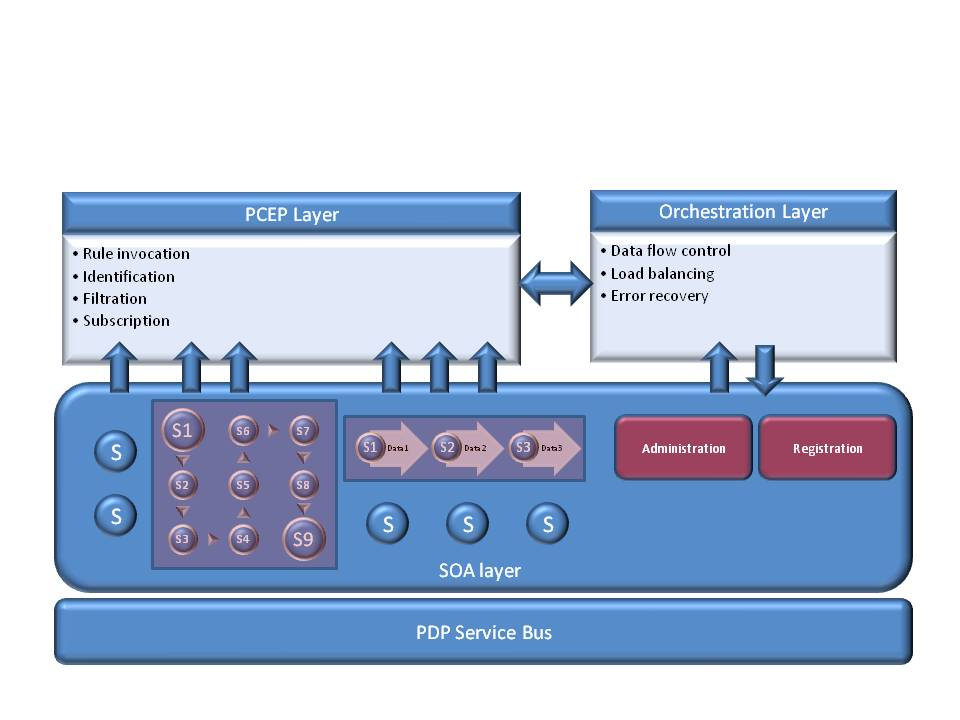
\includegraphics[width=5in]{clara1a.eps} 
\caption{\small{PDP: Physics Data Processing, PCEP: Physics Complex Event Processing, S: Services}}
\label{fig:clara1a}
\end{figure}
%%%%%%%%%%%%%%%%%%%%%%%%%%%%%%%%%%%%%%%%%%%%%%%%%%%%%%%%%%%%%%%%%%%%%%%%

\subsection{The Problem Statement}

Physics data processing application development is a collaborative process. 
On one hand, it involves computer scientists developing framework and basic 
software components, while on the other hand, it calls for physicists to 
develop and implement the specific algorithms needed for simulation, 
reconstruction, calibration, etc.  In addition, there will also be a 
physicist developing the data analysis programs to produce the final physics 
results.  The quality of the physics results depends on the number of 
end-user physicists that are performing and/or cross-checking the physics 
data processing stages. The unprecedented scale and complexity of the physics 
computing environment requires substantial software engineering skills from 
the end-user physicist.  As a result, we have a reduced number of qualified 
data processing physicists, resulting in a poor physics outcome. 
The {\tt CLAS12} computing environment must keep up with fast-growing 
computing technologies.  Taking into account the long lifetime of the physics 
data processing applications, we must organize software in a way that permits 
including or discarding some of the software technologies in an easy way, 
without major reorganization and/or redesign.

\subsubsection{Physics Data Processing Environment}

We have categorized three groups of people working with the framework. This 
categorization is not intended to be exclusive and it is a categorization of 
interaction rather than of people, since many people will belong to several 
groups.

\begin{itemize}

\item {\bf A. Framework developers:} These people are responsible for the 
design, implementation, and maintenance of the framework itself. 

\item {\bf B. Physics application software developers:} This group of people 
will be required to have strong computing skills and more knowledge of the 
framework than what is required by the average physicist user.

\item {\bf C. Framework users:} These people are primarily interested in 
getting physics results.  Using human machine interfaces they compose desired 
physics data processing applications and produce histograms, statistical 
distributions, etc.
\end{itemize}

Our goal is to widen group C and make this group less dependent on the 
support of the A and B groups. 

\subsubsection{Design Requirements}

\begin{itemize}
\item The framework shall be simple to use and easy to learn.
\item The framework should be customizable to be able to adapt to the 
different data processing tasks.
\item The framework shall provide context-sensitive help and assistance, with 
many real-world physics data processing application examples.
\item The framework shall provide ready-to-use modules, encapsulating 
essential functionalities of the physics data processing system.
\item The modules shall be reusable and easily replaceable.
\item Physics data processing application design and implementation shall 
require a few or no programming skills.
\item Neither a specific computing environment nor compiling shall be 
necessary to build and run physics data processing applications.
\item The framework shall provide a graphical environment for physics data 
processing application development.
\item The framework shall be network distributed and shall have temporal 
continuity.
\item The new system shall provide web access to the framework for remote 
configuration and execution of the data processing applications. The 
necessary security considerations must be addressed. 
\end{itemize}

\subsection{SOA}

ClaRa identifies the physics data processing application as a composite 
application. A composite application is an application that is both assembled 
and orchestrated. An assembly is a process of combining together many 
different pieces into a workable unit, and an orchestration is making sure 
that those pieces work together collaboratively with one another to solve the 
given problem in a given scenario. Composite applications are known to be more 
efficient, robust, and flexible. Composites of the software application known 
as software services are more specialized, easily maintainable, and easily 
replaceable and modifiable. Therefore software applications, composed of 
software services are extremely flexible, robust, and adaptable to address 
different data processing needs. The SOA provides the foundation for 
creating, deploying, maintaining, and governing the software services. The 
ClaRa framework is the implementation of the SOA architecture.

\subsubsection{Design Strategies}

ClaRA adopts data centric approach, concentrating its main focus on a data that is moving and transforming in the system. 
Its the data flow that defines the essential aspect of the physics data processing application.
%The ClaRa framework provides guidelines, policies, and approaches for how 
%physics data processing services are designed, deployed, and managed. 
ClaRa services communicate with each other through message passing.  The
framework supports two distinct messaging protocols and transports: cMsg over 
TCP/IP and SOAP over HTTP. The services, using cMsg proprietary 
publish-subscribe messaging protocol are designed to compose performance 
critical applications, and do not require special security considerations. 

\subsubsection{Classification of the Services}

ClaRa design guidelines are based on adopted design strategic decisions. In 
order to optimize service communications and service clustering, ClaRa 
suggests separation between algorithm and data services. For example 
{\it cluster finder} is an example of the algorithmic service and 
{\it hits in the calorimeter} is a data service. ClaRa further categorizes 
data services into three categories: event, detector, and statistical data 
services. Also standard data exchange format is used between services. 
EVIO data format is used for data exchange between services.  ClaRa 
supports flexible segmentation of the data processing application. In the 
very coarse level of segmentation, a service is not different then a large 
monolithic software application. In this case the ClaRa framework plays the 
role of a process manager and controller.  Fig.~\ref{fig:clara2} illustrates 
an example of a tracking application service composition.

%%%%%%%%%%%%%%%%%%%%%%%%%%%%%%%%%%%%%%%%%%%%%%%%%%%%%%%%%%%%%%%%%%%%%%%%
\begin{figure}[htbp]
\centering
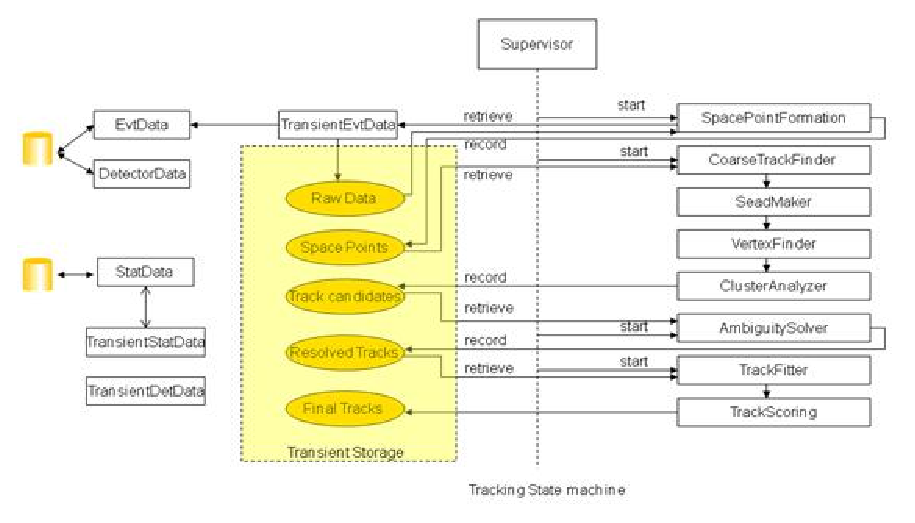
\includegraphics[width=6in]{clara2.eps} 
\caption{\small{Service decomposition of a hypothetical tracking 
application.  Ovals represent in-memory data storage and rectangles 
represent services. Supervisor is the service that orchestrates the 
tracking application.}}
\label{fig:clara2}
\end{figure}
%%%%%%%%%%%%%%%%%%%%%%%%%%%%%%%%%%%%%%%%%%%%%%%%%%%%%%%%%%%%%%%%%%%%%%%%

\subsubsection{Performance Measurements}

Integration and coordination in real-time data and information from 
network-distributed services will clearly carry performance penalties.  It 
is also obvious that poor decomposition of the physics data processing 
application in terms of granularity can largely affect composed application 
performance.   

%%%%%%%%%%%%%%%%%%%%%%%%%%%%%%%%%%%%%%%%%%%%%%%%%%%%%%%%%%%%%%%%%%%%%%%%
%\begin{figure}[htbp]
%\centering
%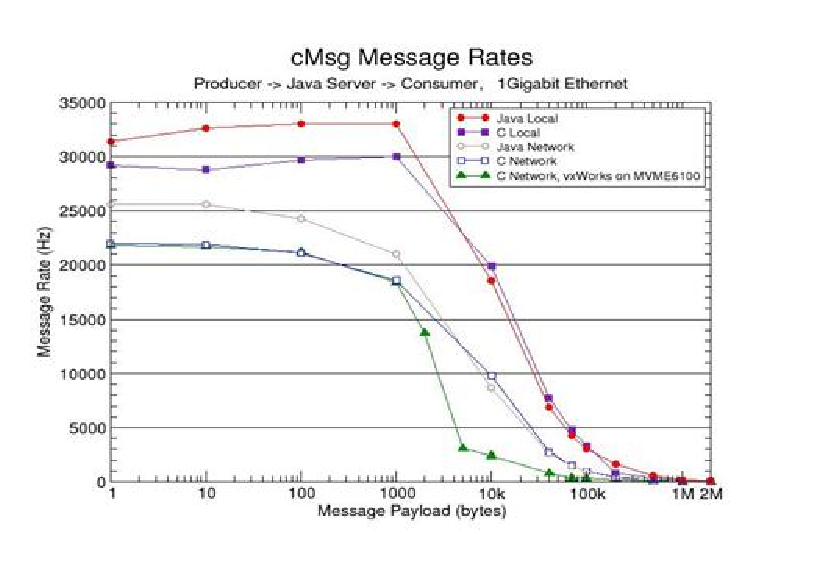
\includegraphics[width=5in]{clara3.eps} 
%\caption{cMsg measured performance.}
%\label{fig:clara3}
%\end{figure}
%%%%%%%%%%%%%%%%%%%%%%%%%%%%%%%%%%%%%%%%%%%%%%%%%%%%%%%%%%%%%%%%%%%%%%%%
 
\subsection{Web Services}

ClaRa web services are developed using J2EE (Java Enterprise Edition) JAX 
WS 2.0.  Currently all the ClaRa cMsg services written in Java are also 
deployed as a ClaRa Web Service.  The ClaRa Web Services platform makes 
{\tt CLAS12} services programmatically accessible over standard Internet 
protocols.

\section{Services}

\subsection{Authentication}

Services, by their nature, are accessible to remote clients. While the 
ultimate security policy for {\tt CLAS12} has not been addressed, the 
software group recognizes that some form of user authentication will be 
required. The authentication service will allow other services to ask 
whether or not a given user is authorized to receive the information  
requested.

There are number of ways to implement such a service, including some 
powerful but platform-specific solutions, such as the authentication suite 
provided by Microsoft .NET. Again, the loose coupling provide by a 
Service-Oriented Architecture allows us to define the authentication 
interface contract even before we decide on an implementation, and it 
allows us to replace implementations to meet growing needs to address 
unforeseen security concerns.

So we plan to start with an authentication service that will accept a 
username and password, and return an integer value for the user's access 
level. (We may only ever need a no access/full access determination.) The 
first implementation of the service will just return a value indicating 
full access for all requests. That will allow other services to build in 
their authentication request. From there we will move to an actual 
implantation, perhaps one using an LDAP or MySQL server that stores username, 
passwords, and access levels. That may prove sufficient, but if not, we can 
always migrate to an even more secure authentication scheme without breaking 
the framework.

\subsection{Detector Geometry}

The geometry service is an example of the Detector Data Service. This is 
the front-end of the {\tt CLAS12} geometry data, encapsulating data access 
and data management details from the service consumers. All the ClaRa 
algorithm services, including simulation, reconstruction, alignment, etc., 
access the geometry service using standard service communication protocols, 
provided by the framework. Currently geometry information is stored in the 
MySQL database, but in the future we might consider changing the geometry 
data storage technology (for example XML), however all of this will be
fully transparent to the geometry service consumers.

\subsection{Event Display}

The single event display in the {\tt CLAS12} framework will be both a 
service consumer (a client) and a service provider.  Implementing the 
event display as a service consumer provides all the benefits discussed in 
the section on Service-Oriented Architecture. Additionally, it allows us to 
use the thin-client model favored by modern software architects. Thin 
clients, sometimes called smart clients, split their application code 
between data models and processing, performed as much as possible in a 
different thread, process or CPU, and visualization. This shrinks the pure 
visualization code, allowing it to be deployed remotely or updated frequently 
without incurring a huge download penalty. The most familiar and successful 
model is probably Google Earth. A thin client is downloaded and runs quickly, 
but complicated imagery processing is performed remotely. 

A Service-Oriented Architecture is one way to implement thin clients. As 
much as possible, without hampering performance, no visualization processing, 
such as acquiring detector geometry, is performed by a service and the thin 
client obtains the geometry by sending a request.

In the case of the event display (see Fig.~\ref{fig:eventDisplay}), the 
client will use a variety of services, such as geometry, magnetic field, 
event streaming, file system access, run metadata, and analysis. It will 
also be a service provider through a display service.  One service it will 
provide will include simple pictures of random online events so that remote 
users, for diagnostic purposes, can see pictures of recent events. Another 
more sophisticated service will be to answer a request for an image of a 
specific event viewed in a certain way, such as zoomed in on Region~1 in 
Sector~3.

%%%%%%%%%%%%%%%%%%%%%%%%%%%%%%%%%%%%%%%%%%%%%%%%%%%%%%%%%%%%%%%%%%%%%%%%
\begin{figure}[htbp]
\centering
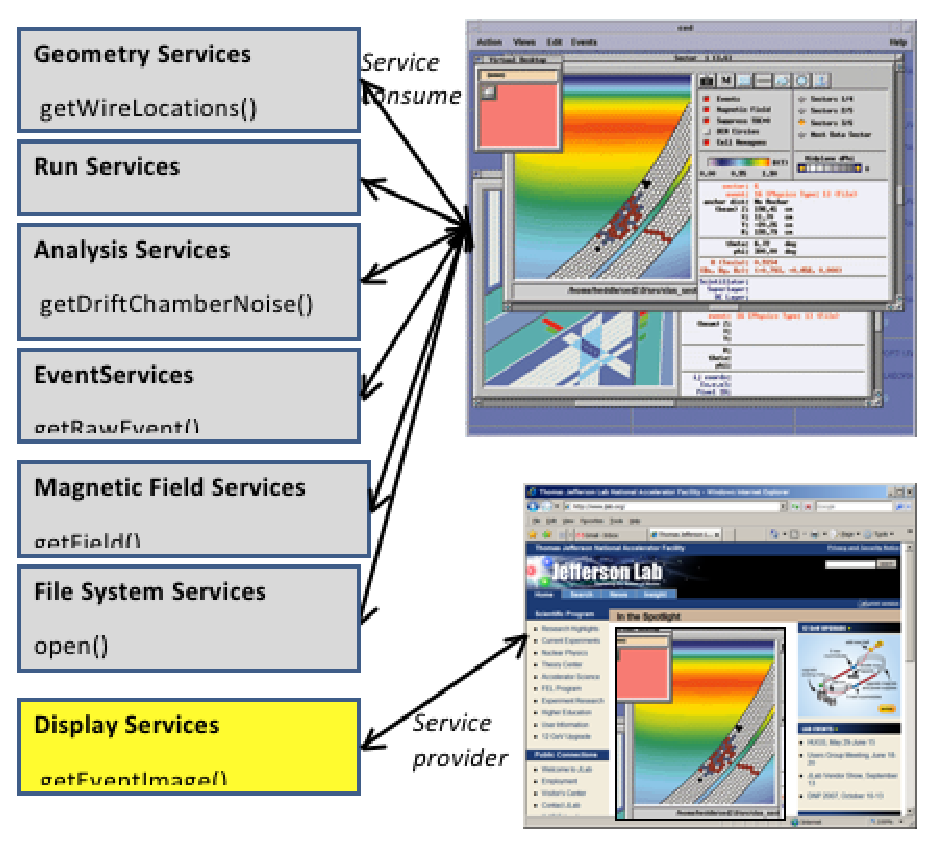
\includegraphics[width=5in]{eventDisplay.eps} 
\caption{\small{The event display will consume a number of {\tt CLAS12} 
services. It will also provide a display service.}}
\label{fig:eventDisplay}
\end{figure}
%%%%%%%%%%%%%%%%%%%%%%%%%%%%%%%%%%%%%%%%%%%%%%%%%%%%%%%%%%%%%%%%%%%%%%%%

Another feature of the event display is that it will employ a plug-in 
architecture based on the reflection capabilities of the JAVA language. 
This will provide a simple yet powerful extendibility feature for users who 
would like to use the event display to visualize and debug their new analysis 
and simulation code. Reflection is a way that JAVA applications can examine 
all the classes in their path. The event display will look for all classes 
that inherit from a specific abstract base class. Once found, the application 
will create an object from that class and then provide a set of services for 
the object, such as notifying it that a new event has arrived. 

In this scheme, neither recompilation or even restart of the event display is 
required.  The developer extending the event display creates the class, drops 
it into the path, and the class will be plugged-in to the application. If the 
plug-in proves of general use, it can be placed in the path of the shared 
event display (e.g., the run in the counting house) and all users will have 
access.  However, if it is found to be an undesirable feature, the class file 
can simply be deleted.  All of this adding and removing of features will 
occur with no changes to the code or recompilation of the base event display. 

\subsection{Data and Algorithm Services}

In addition to our purpose to produce a Service-Oriented Architecture based 
design, we have decided to separate data services from algorithm services. 
An algorithm service, in general, will accept and process an output data 
object from a data service and will then produce a new data object.

\subsubsection{Basic Types of Data Services}

One of our main design choices is to separate data services dealing with the 
data objects that are resident on the disk from the data services that 
manipulate the data objects in memory.  An objective that we would like 
to achieve is to make algorithm services independent of the technology we 
use for data object persistency. This will allow replacing outdated 
persistency technology in the future without affecting user-produced 
algorithm services. By separating persistent and transient data services we 
also hope to achieve a higher level of optimization by targeting inherently 
different optimization criteria for persistent and transient data storages. 
For example, regarding the data objects on the disk, one should invest more 
effort to optimize I/O performance, data size, avoid multiple I/O requests, 
etc. On the other hand, for the transient data in the memory, we should 
achieve highly optimized execution performance, APIs, and usage simplicity.

We foresee three major categories of data objects:

\begin{itemize}
\item Event data, such as raw data, simulated data, reconstructed data, etc.
\item Detector data, describing a detector apparatus in order to interpret 
the event data. Examples of the detector data are geometry data, calibration 
data, alignment data, slow controls data, etc.
\item Statistical data (histograms, n-tuples, etc.)
\end{itemize}

Specific data services are provided for each of these data categories (see 
Fig.~\ref{fig:service1}).

%%%%%%%%%%%%%%%%%%%%%%%%%%%%%%%%%%%%%%%%%%%%%%%%%%%%%%%%%%%%%%%%%%%%%%%%
\begin{figure}[htbp]
\centering
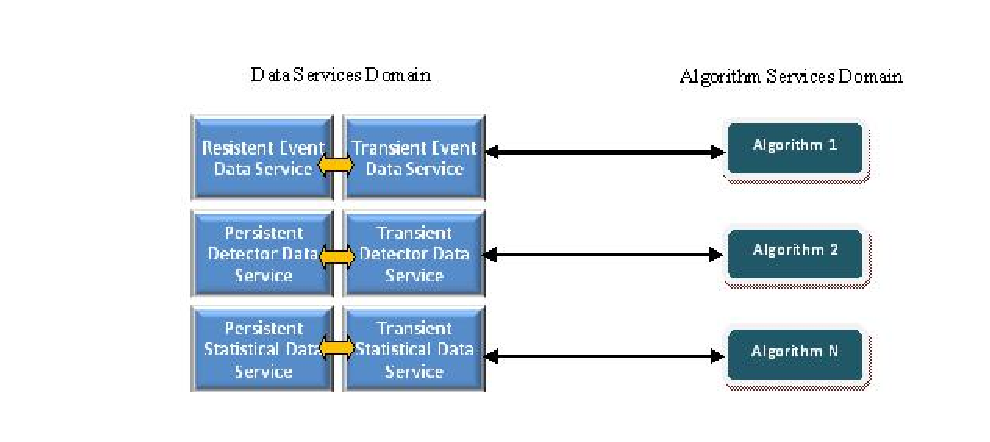
\includegraphics[width=6in]{service1.eps} 
\caption{\small{Different data services in the ClaRa framework. Algorithm 
services deal with transient data services only.}}
\label{fig:service1}
\end{figure}
%%%%%%%%%%%%%%%%%%%%%%%%%%%%%%%%%%%%%%%%%%%%%%%%%%%%%%%%%%%%%%%%%%%%%%%%

\subsection{Magnetic Field}

The magnetic field service is implemented in c++ with extensive use of 
the standard library's map construct.  The entire field map is divided 
into individual maps corresponding to various magnets such as the solenoid 
and main torus.  In addition, it has methods to get the magnetic field at 
a certain point, check for consistency within the map, and interpolate values 
inside the defined grid spacing.

Each map can be tailored to the field it holds. For instance, the main torus 
is defined in cylindrical coordinates, with $\phi\in[0,\frac{\pi}{6}]$.  The 
class holding the main torus map then has an algorithm to calculate the field 
at any point $\phi\in[0,2\pi]$.  However, this is only good for ideal fields. 
For measured fields, the class can be easily extended to handle a case where 
the field is known precisely in the entire region.  Furthermore, the 
dimensions and coordinates of the map's position and field need not be same.
Inside the solenoid field for instance, the position is stored in ($r$,$\phi$),
while the magnetic field is stored in ($x$, $y$, $z$).

A separate \emph{mother} class is responsible for loading in and storing the 
maps from a database or file. This class is aware of the volumes of the 
individual maps and sums the fields where appropriate.

The final layer on this system is the magnetic field ClaRa service. This is 
where the mother class is initialized and held in memory. Several mother 
classes can be held; i.e. one for the ideal fields, one for the measured 
fields, and one mix of these two. The service registers itself with the 
ClaRa system and can provide the various field maps in several formats 
depending on the consumer's preference.  As an example, the service can be 
polled for an entire map or for an individual position.


The CLAS 12 GeV torus field is in the ASCII file sptorus\_map.dat. This file is 495.5 MB (Aside: the gzipped version is 110 MB. 
We should in fact place the gzipped file in the SVN repository otherwise there is no blessed location where sptorus\_map.dat is available).

The format of sptorus\_map.dat is: 

\begin{itemize}
    \item $\phi$ varies from $0.0^\circ$ to $30.0^\circ$ in steps of $0.25^\circ$.
    \item $r$ varies from 0.0 to 500 cm in steps of 2.0 cm.
    \item $z$ varies from 100.0 cm to 600.0 cm in steps of 2.0 cm
    \item The field values are in kG, and are provided in Cartesian components.
\end{itemize}
 

That is the (uniform) grid is cylindrical coordinates, and the field is Cartesian. 
Each line in the file has six numbers: $\phi_i$, $r_j$, $z_k$, $B_x$, $B_y$, $B_z$. 
The loop over $z$ is the inner (fastest) loop. 
The $r$-loop is the middle, and the $\phi$-loop is the outer, slowest varying loop. 
While the ASCII map is useful, it is way too slow to read for frequent use. We need to create a binary version
which contains a twenty-member, 32-bit word header. (The 80 bytes for this header is in the noise when it comes file size.) The proposed format is
shown in Table \ref{magfieldfileheader}.

\begin{table}[t!]
\begin{center}
\begin{tabular}{|l|}\hline
(int) 0xced (decimal: 3309) magic number\u2014to check for byte swapping \\[2pt] \hline
(int) Grid Coordinate System (0 = cylindrical, 1 = Cartesian) \\[2pt] \hline
(int) Field Coordinate System (0 = cylindrical, 1 = Cartesian) \\[2pt] \hline
(int) Length units (0 = cm, 1 = m) \\[2pt] \hline
(int) Angular units (0 = decimal degrees, 1 = radians) \\[2pt] \hline
(int) Field units (0 = kG, 1 = G, 2 = T) \\[2pt] \hline
(int) q1 min (min value of slowest varying coordinate) \\[2pt] \hline
(int) q1 max (max value of slowest varying coordinate) \\[2pt] \hline
(int) Nq1 number of points (equally spaced) in q1 direction \\[2pt] \hline
(float) q2 min (min value of medium varying coordinate) \\[2pt] \hline
(float) q2 max (max value of medium varying coordinate) \\[2pt] \hline
(int) Nq2 number of points (equally spaced) in q2 direction \\[2pt] \hline
(float) q3 min (min value of fastest varying coordinate) \\[2pt] \hline
(float) q3 max (max value of fastest varying coordinate) \\[2pt] \hline
(int) Nq3 number of points (equally spaced) in q3 direction \\[2pt] \hline
Reserved 1 \\[2pt] \hline
Reserved 2 \\[2pt] \hline
Reserved 3 \\[2pt] \hline
Reserved 4 \\[2pt] \hline
Reserved 5 \\[2pt] \hline
\end{tabular}
\caption{Proposed header format for magnetic field, binary file.}\label{magfieldfileheader}
\end{center}
\end{table}
 
 The only ambiguity is the meaning of the triplet $(q_1, q_2, q_3)$. 
For cylindrical coordinates, to be compatible with sptorus\_map.dat, the triplet means {$\phi$, $r$, $z$}. 
It seems most natural that for Cartesian coordinates the triplet maps to: $(x, y, z)$. 
Thus for a Cartesian field map, $x$ would be the outer, slowest-varying grid component.
The total number of field points will be: $N = N1\times N2\times N3$ and we will store floats, not doubles. 
Each point requires three four-byte quantities. The total size of the binary file will be $80 + 3\times 4\times N$.
The step size in direction $i$ is $(q_{imax} - q_{imin})/(N_i - 1)$.
The reserved fields can be used, in some manner to be defined, to indicate scaling or the application of a smoothing function.
The field follows the header, in repeating triplets shown in Table \ref{reservedfields}.
\begin{table}[t!]
\begin{center}
\begin{tabular}{|c|}\hline
B1 \\[2pt]\hline
B2 \\[2pt]\hline
B3 \\[2pt]\hline
\end{tabular}
\caption{Reserved fields for magnetic field header.}\label{reservedfields}
\end{center}
\end{table}
The first three entries correspond to the field components for the first grid point, the next three for the second grid point, etc. The ordering, for consistency, should be:

$(B_x, B_y, B_z)$ if the field is Cartesian

$(B_\phi, B_r, B_z)$ if the field is Cylindrical

\noindent For the binary version of the standard file sptorus\_map.dat, we have for the header shown in Table \ref{magfieldfileheader2}.
Thus the three step sizes are:

$\Delta\phi = (30-0)/(121-1) = 0.25^\circ$

$\Delta r = (500-0)/(251-1) = 2~ cm$

$\Delta z = (600-100)/(251-1) = 2~ cm$

\noindent The size of the binary is $80 + 3\times4\times121\times251\times251 = 91,477,532~ bytes$.

\begin{table}[b!]
\begin{center}
\begin{tabular}{|l|}\hline
0xced  \\[2pt] \hline
0 (grid is cylindrical) \\[2pt] \hline
1 (field is Cartesian) \\[2pt] \hline
0 (units: cm) \\[2pt] \hline
0 (units: decimal degrees) \\[2pt] \hline
0 (units: kG) \\[2pt] \hline
0.0 ($\phi_{min}$) \\[2pt] \hline
30.0 ($\phi_{max}$, degrees) \\[2pt] \hline
121 ($N_\phi$) \\[2pt] \hline
0.0 ($r_{min}$) \\[2pt] \hline
500.0 ($r_{max}$, cm) \\[2pt] \hline
251 ($N_r$) \\[2pt] \hline
100.0 ($z_{min}$, cm) \\[2pt] \hline
600.0 ($z_{max}$, cm) \\[2pt] \hline
251 ($N_z$) \\[2pt] \hline
0 (Reserved 1) \\[2pt] \hline
0 (Reserved 2) \\[2pt] \hline
0 (Reserved 3) \\[2pt] \hline
0 (Reserved 4) \\[2pt] \hline
0 (Reserved 5) \\[2pt] \hline
\end{tabular}
\caption{Example of header contents for magnetic field, binary file.}\label{magfieldfileheader2}
\end{center}
\end{table}




\section{Simulation}

There are two different, though overlapping, areas in our current simulation 
effort. One is focused on validating design decisions for the upgraded 
detector, the other on building a modern simulation system that can be used 
for the life of the {\tt CLAS12} program. The former has two components: (1) a 
parametric Monte Carlo that can estimate the resolution for charged particle 
tracking and (2) a full GEANT3 system that depends on the code base that has 
been developed for the current {\tt CLAS} detector, modified to reflect the 
new design, including reconstruction. The latter is an entirely new 
GEANT4-based, object-oriented design.

\subsection{Parametric Monte Carlo}

One of the fundamental algorithmic challenges in the design of {\tt CLAS12} 
is the problem of track reconstruction in a non-uniform magnetic field.  Not 
only does the torus produce an inhomogeneous field in the tracking volume, 
but charged particles emerging from the solenoid must be tracked as they 
traverse the fringe field of that magnet. Since no analytic form for the 
particle trajectories exist, they must be calculated by ``swimming'' the
particles numerically through a map of the magnetic field. Track fitting 
then becomes very expensive in terms of CPU time. One way to finesse the 
problem is to linearize it by parameterizing the trajectory as small 
deviations from a reference trajectory. The reference trajectory must come 
from a ``swim'', but subsequent ``trial'' trajectories, with different 
starting parameters (momentum, direction), can be computed by a simple matrix 
inversion. Position resolution is put in at a set of idealized detector 
planes. It is also possible to incorporate multiple Coulomb scattering in 
this model. This technique has already been used to estimate momentum 
resolution for {\tt CLAS12}. Results appear in other sections of this 
document.  The method cannot give information on some things, such as the 
effect of accidentals, track reconstruction efficiency or confusion due to 
overlapping tracks.

\subsection{{\tt CLAS} Software with the {\tt CLAS12} Geometry}

The current {\tt CLAS} system consists of over half a million lines of 
FORTRAN, c, and c++ code contained in about 2,500 source code files. It 
represents a large investment by the {\tt CLAS} collaboration over many 
years. {\tt CLAS}, with its toroidal magnetic field, also presents the 
difficulty of tracking in an inhomogeneous field and that problem has 
been solved in this body of code.  Recently, the geometry of crucial detector 
elements was changed to reflect the {\tt CLAS12} design, both in simulation 
and in reconstruction. The resulting system can now do a full GEANT3-based 
simulation and reconstruction of {\tt CLAS12} events, in particular charged 
particle tracking in the forward drift chambers. Studies using this system 
have been carried out to verify momentum resolution results from the 
parametric Monte Carlo and to estimate the effect of accidental M{\o}ller 
scattering background on track reconstruction. More of the details of the 
detector subsystems and beam line components of the upgraded configuration 
are being added to extend the range of these and similar studies.

\subsection{GEANT4 Object-Oriented Detector Simulation}

The GEANT4 simulation software for {\tt CLAS12} is called {\tt gemc} 
({\tt GE}ant4 {\tt M}onte{\tt C}arlo).  The parameters that define the 
simulation (i.e. geometry, sensitivity, magnetic fields, output banks, etc.)
are stored in an external database and used at run-time in STL (c++ Standard 
Template Library) objects.  The database currently in use is the MySQL 
database. Other options (e.g. XML) are also available for consideration.

\paragraph{Geometry}

~~

\vskip 0.3cm

\noindent
The GEANT4 volumes are defined as follows:

\begin{itemize}
\item Shapes, dimensions. Boolean operations of shapes.
\item Material, Magnetic Field, Visual attributes, Identity, Sensitivity 
and Hit Process.
\item Placement(s) in space: position, rotation, copy number.
\end{itemize}

\noindent
These parameters are stored in MySQL tables, one table per detector 
(i.e. HTCC, EC, DC, etc.).  At run time, {\tt gemc} reads an XML file 
that specifies which detector to include in the simulation, including 
possible tilts and displacements from the original positions.

\paragraph{{\tt CLAS12} Geometry Implementation}

~~

\vskip 0.3cm

Particular attention is paid in reproducing in {\tt gemc} the design of each 
detector with as much accuracy and as many details as reasonably achievable.
In Fig.~\ref{fig:svt} the SVT GEANT4 representation is shown, while in 
Fig.~\ref{fig:central} is shown the GEANT4 implementation of the various 
central detectors.

%%%%%%%%%%%%%%%%%%%%%%%%%%%%%%%%%%%%%%%%%%%%%%%%%%%%%%%%%%%%%%%%%%%%%%%%
\begin{figure}[h]
\begin{center}
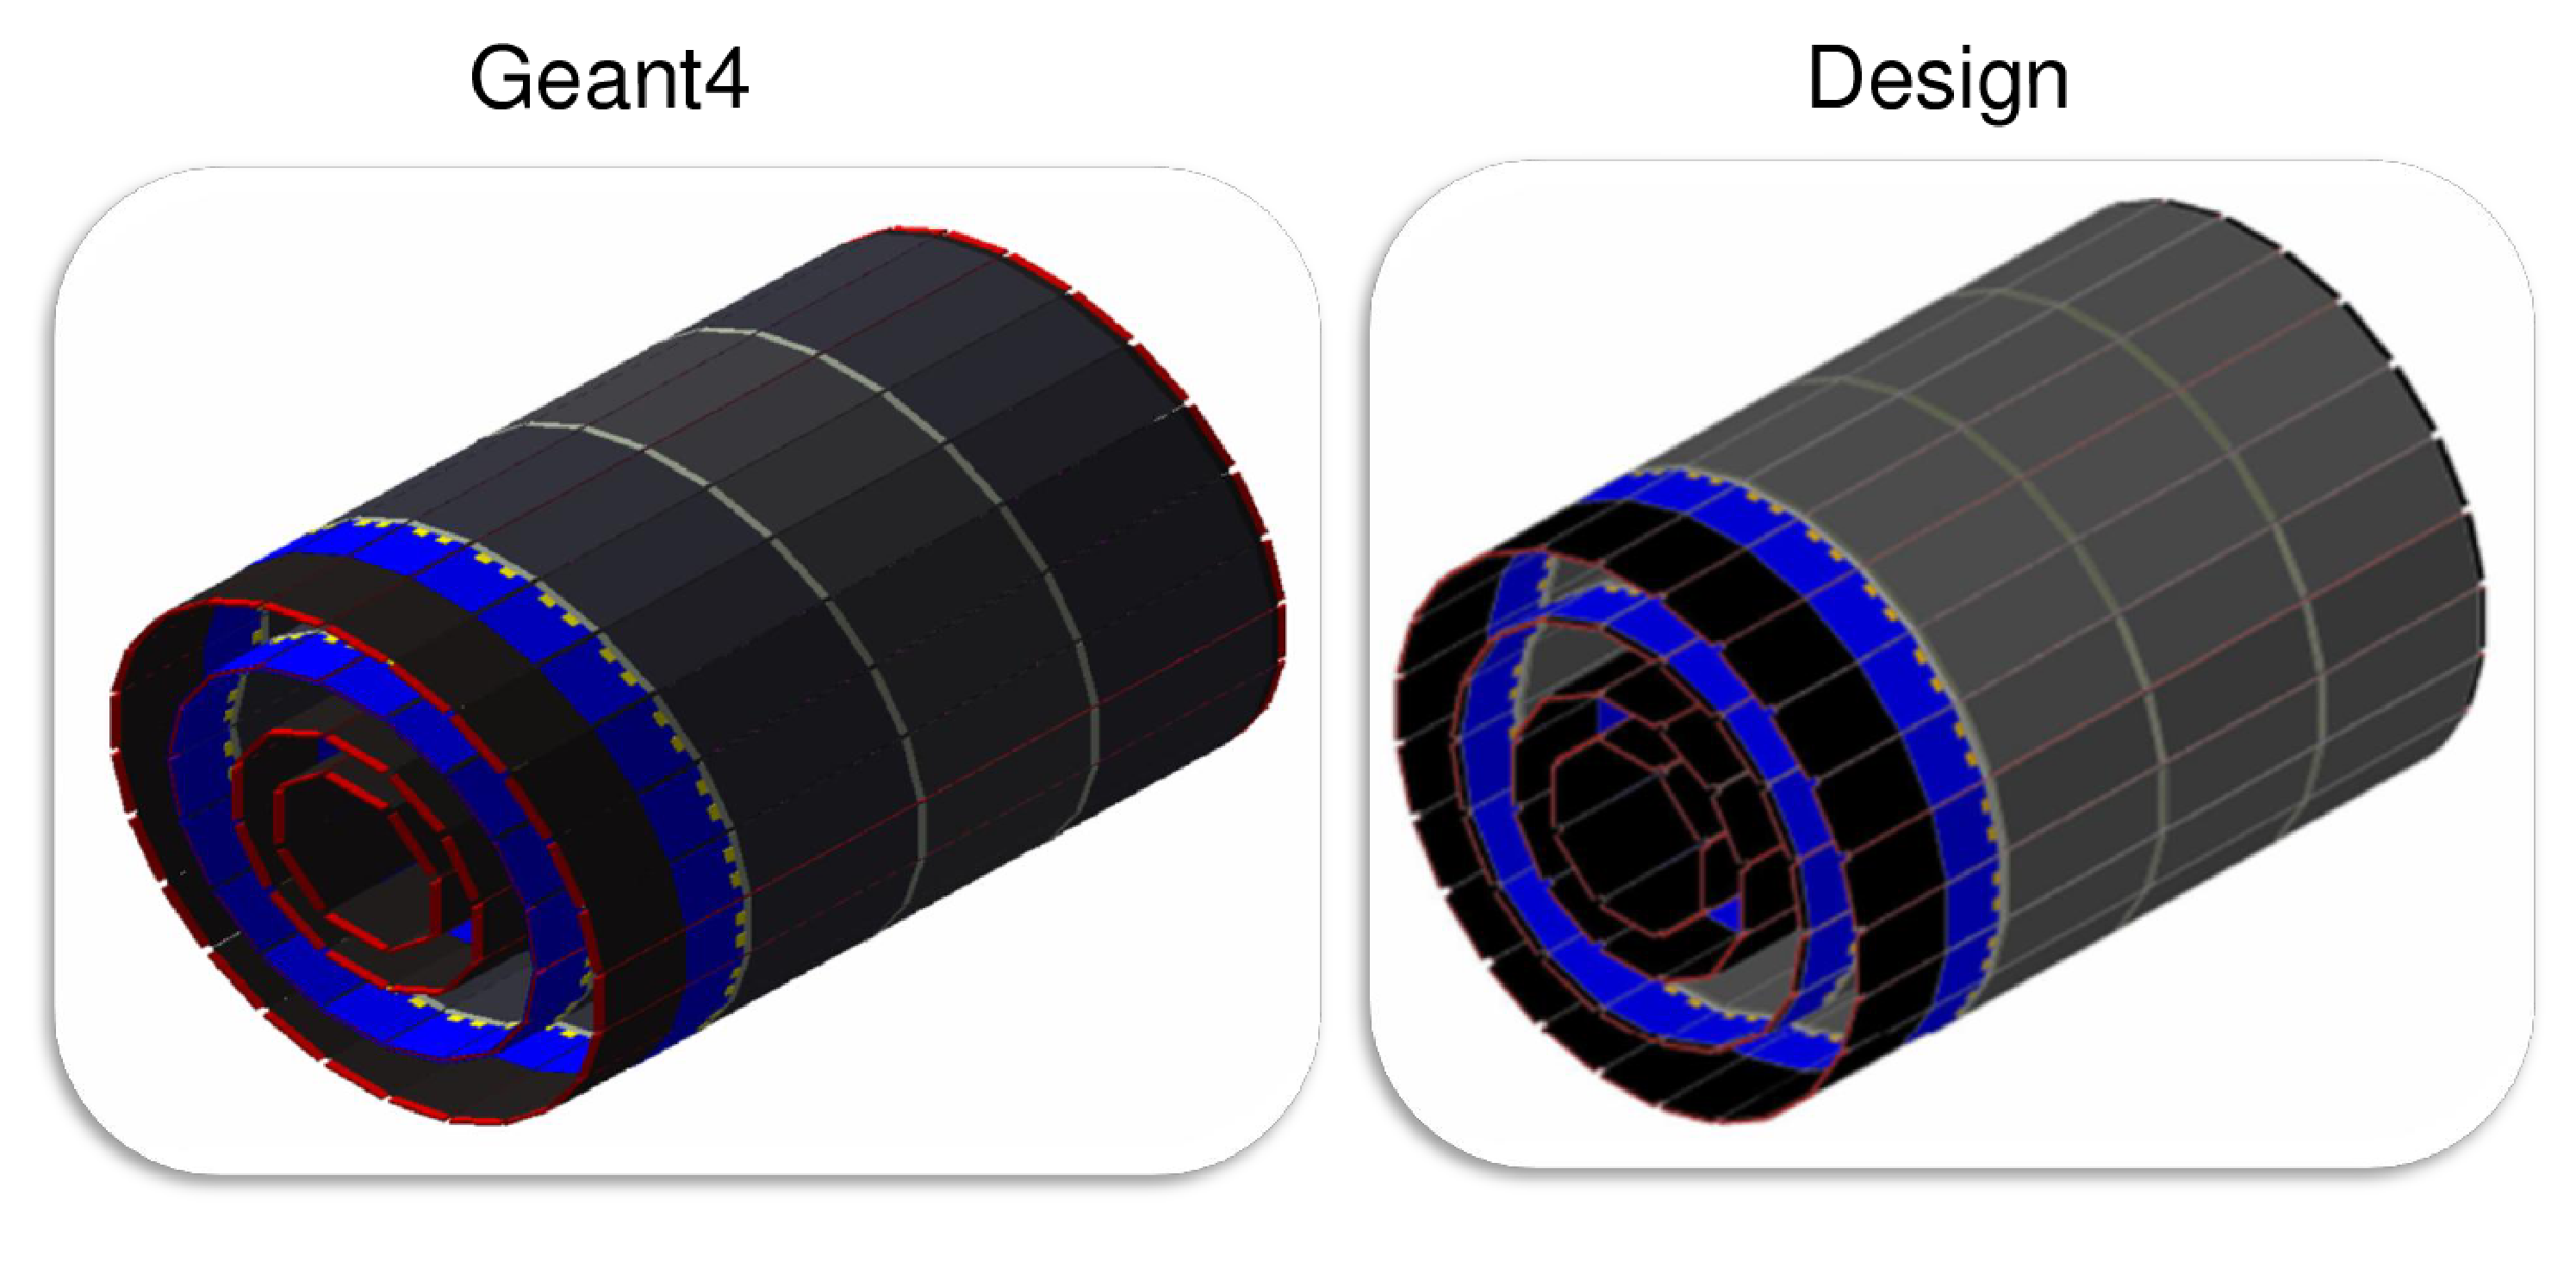
\epsfig{file=bst.eps,width=9.5cm,height=7cm}
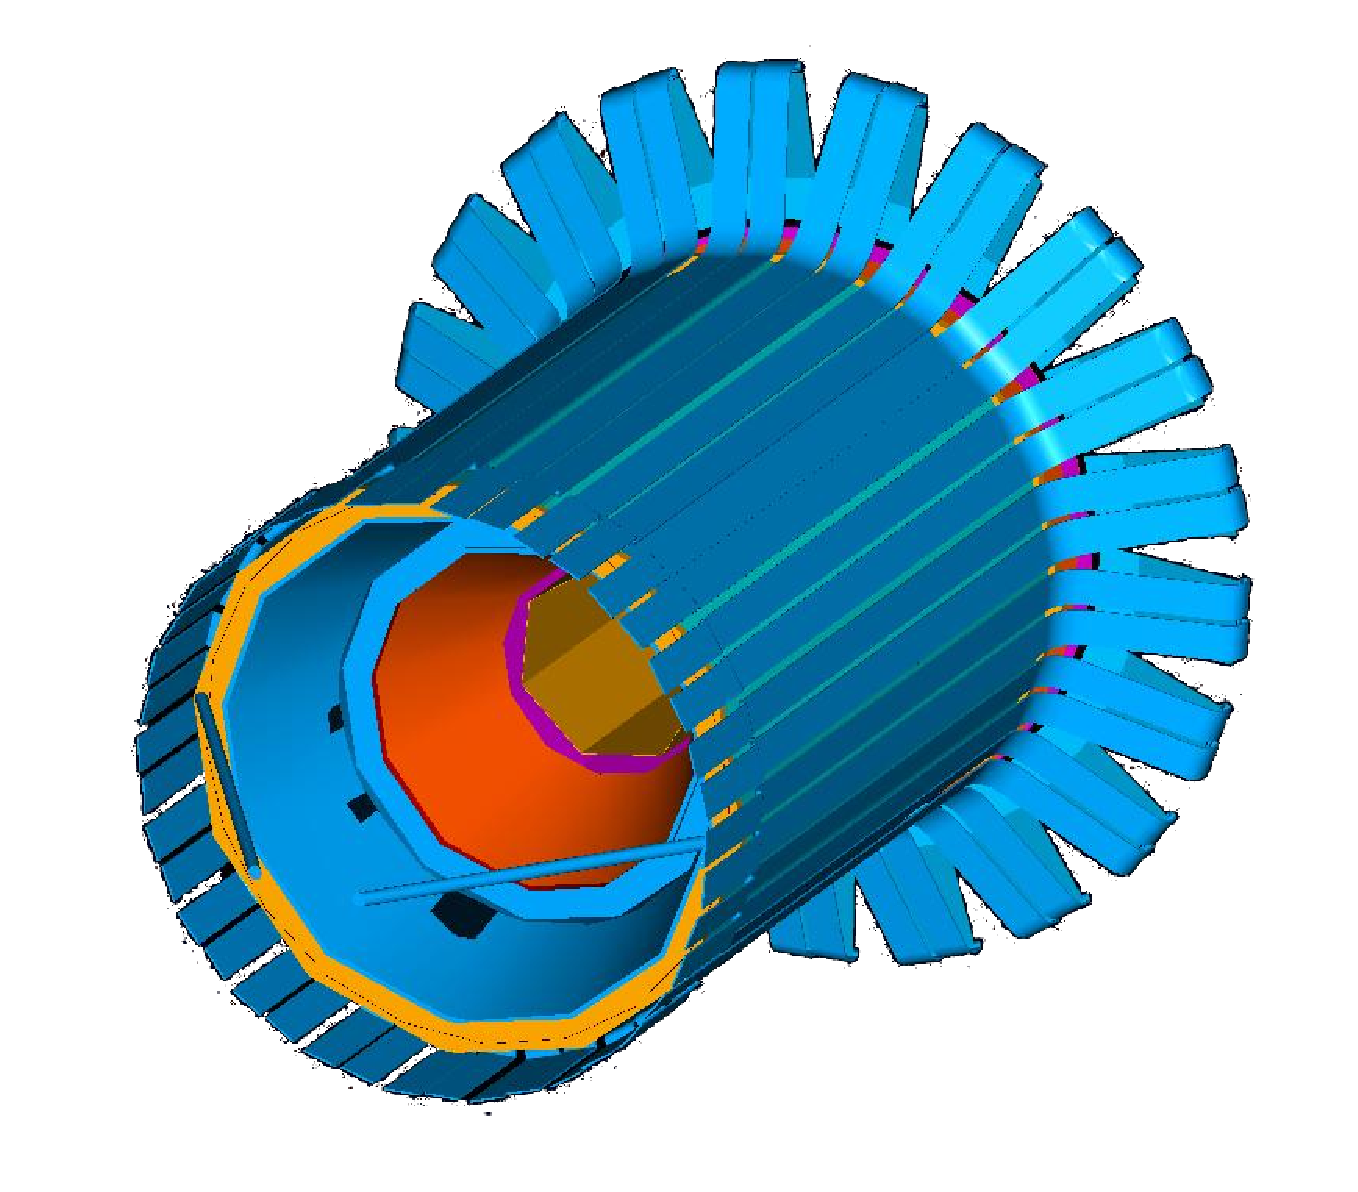
\epsfig{file=svt.eps,width=7.0cm,height=7cm}
\caption{\small{The Silicon Vertex Tracker in GEANT4. (Left) The 
{\tt gemc} BST, (middle) the CAD model BST, and (right) the complete 
{\tt gemc} implementation of the BST+FST.}}
\label{fig:svt}
\end{center}
\end{figure}
%%%%%%%%%%%%%%%%%%%%%%%%%%%%%%%%%%%%%%%%%%%%%%%%%%%%%%%%%%%%%%%%%%%%%%%%
\clearpage
\newpage

%%%%%%%%%%%%%%%%%%%%%%%%%%%%%%%%%%%%%%%%%%%%%%%%%%%%%%%%%%%%%%%%%%%%%%%%
\begin{figure}[h]
\begin{center}
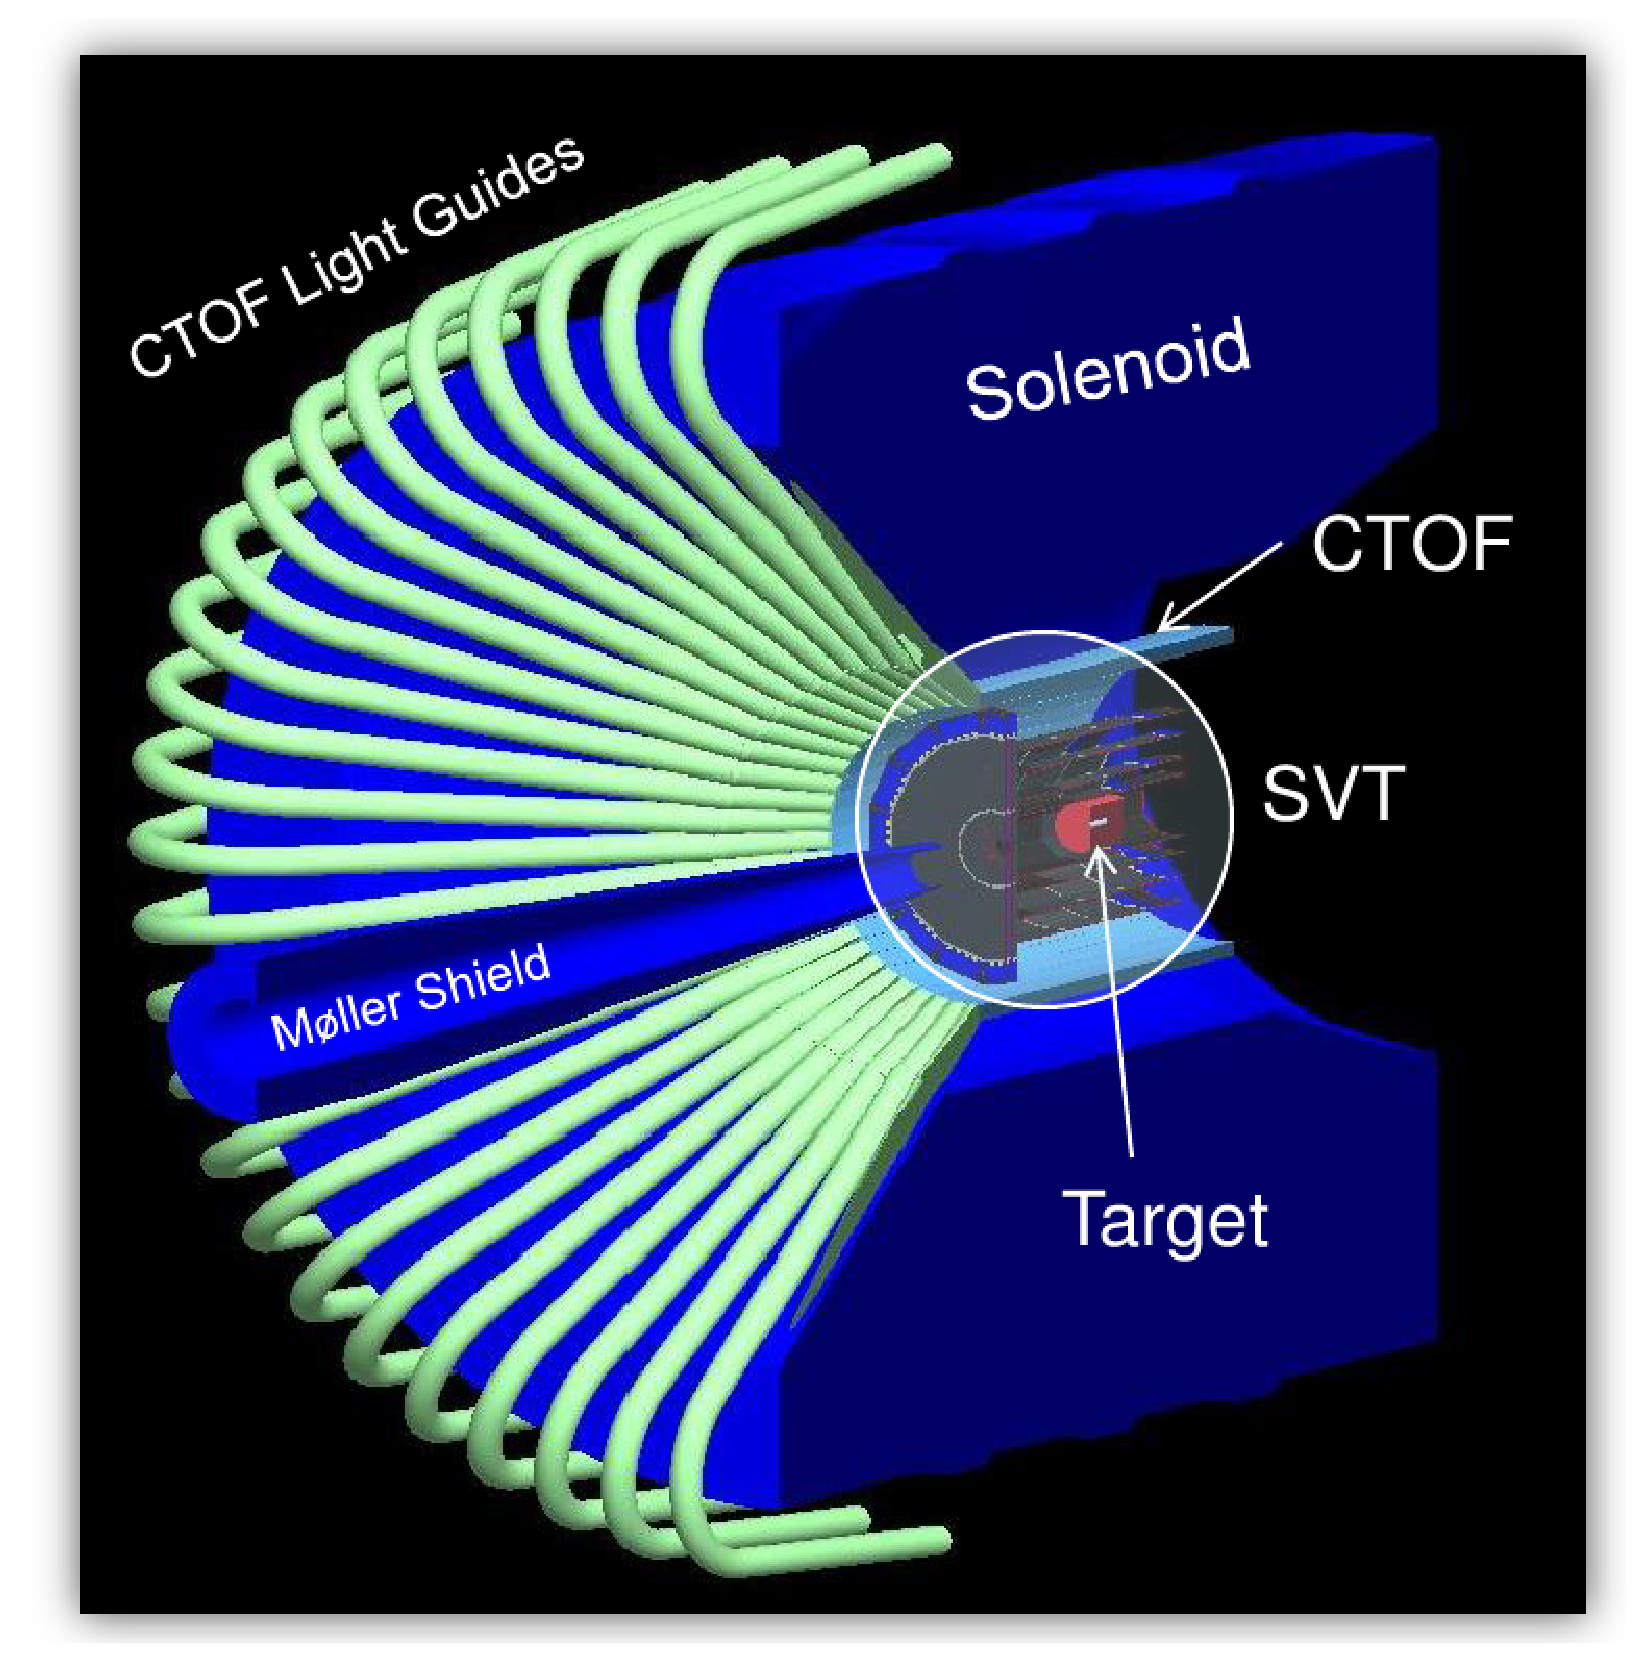
\epsfig{file=central.eps,width=16.0cm,height=16cm}
\caption{\small{The {\tt CLAS12} Central Detector. The target (white) is at 
the {\tt CLAS12} center, surrounded by the SVT (which includes both the
BST and FST) (red).  The CTOF paddles (cyan) are connected to light guides 
(light green) that wrap around the solenoid (blue). The M{\o}ller shield is 
also visible (blue).}}
\label{fig:central}
\end{center}
\end{figure}
%%%%%%%%%%%%%%%%%%%%%%%%%%%%%%%%%%%%%%%%%%%%%%%%%%%%%%%%%%%%%%%%%%%%%%%%

\clearpage
\newpage

\paragraph{Generator}

~~

\vskip 0.3cm

In {\tt gemc} there are two ways to define the primary generator:

\begin{itemize}
\item[1)] {\tt gemc internal generator}: with this method the user defines 
the primary particle type, momentum range, and vertex range.
\item[2)] {\tt external input file}: with this method the user defines 
the format of the input file and the file name.
\end{itemize}

The various file formats are registered in {\tt gemc} by a 
{\it factory method}, which allows derivation of new formats from the 
{\tt gemc} c++ pure virtual methods defined for the input, and to choose 
the desired format at run-time.

In addition to the primary particles, an additional {\it luminosity beam} 
can be defined to add realistic backgrounds to the simulation.  The user 
defines the beam particle type, the number of beam particles per event, and 
the time structure of the beam.

\paragraph{Hit Definition}

~~

\vskip 0.3cm

The {\tt gemc} hit definition is illustrated in Fig.~\ref{fig:hit_def}. A 
{\tt Time Window} (TW) is associated with each sensitive detector. In the 
same detector element, tracks within the TW constitute one hit, while 
tracks separated in time by more than the TW form two separate hits.

%%%%%%%%%%%%%%%%%%%%%%%%%%%%%%%%%%%%%%%%%%%%%%%%%%%%%%%%%%%%%%%%%%%%%%%%
\begin{figure}[h]
\begin{center}
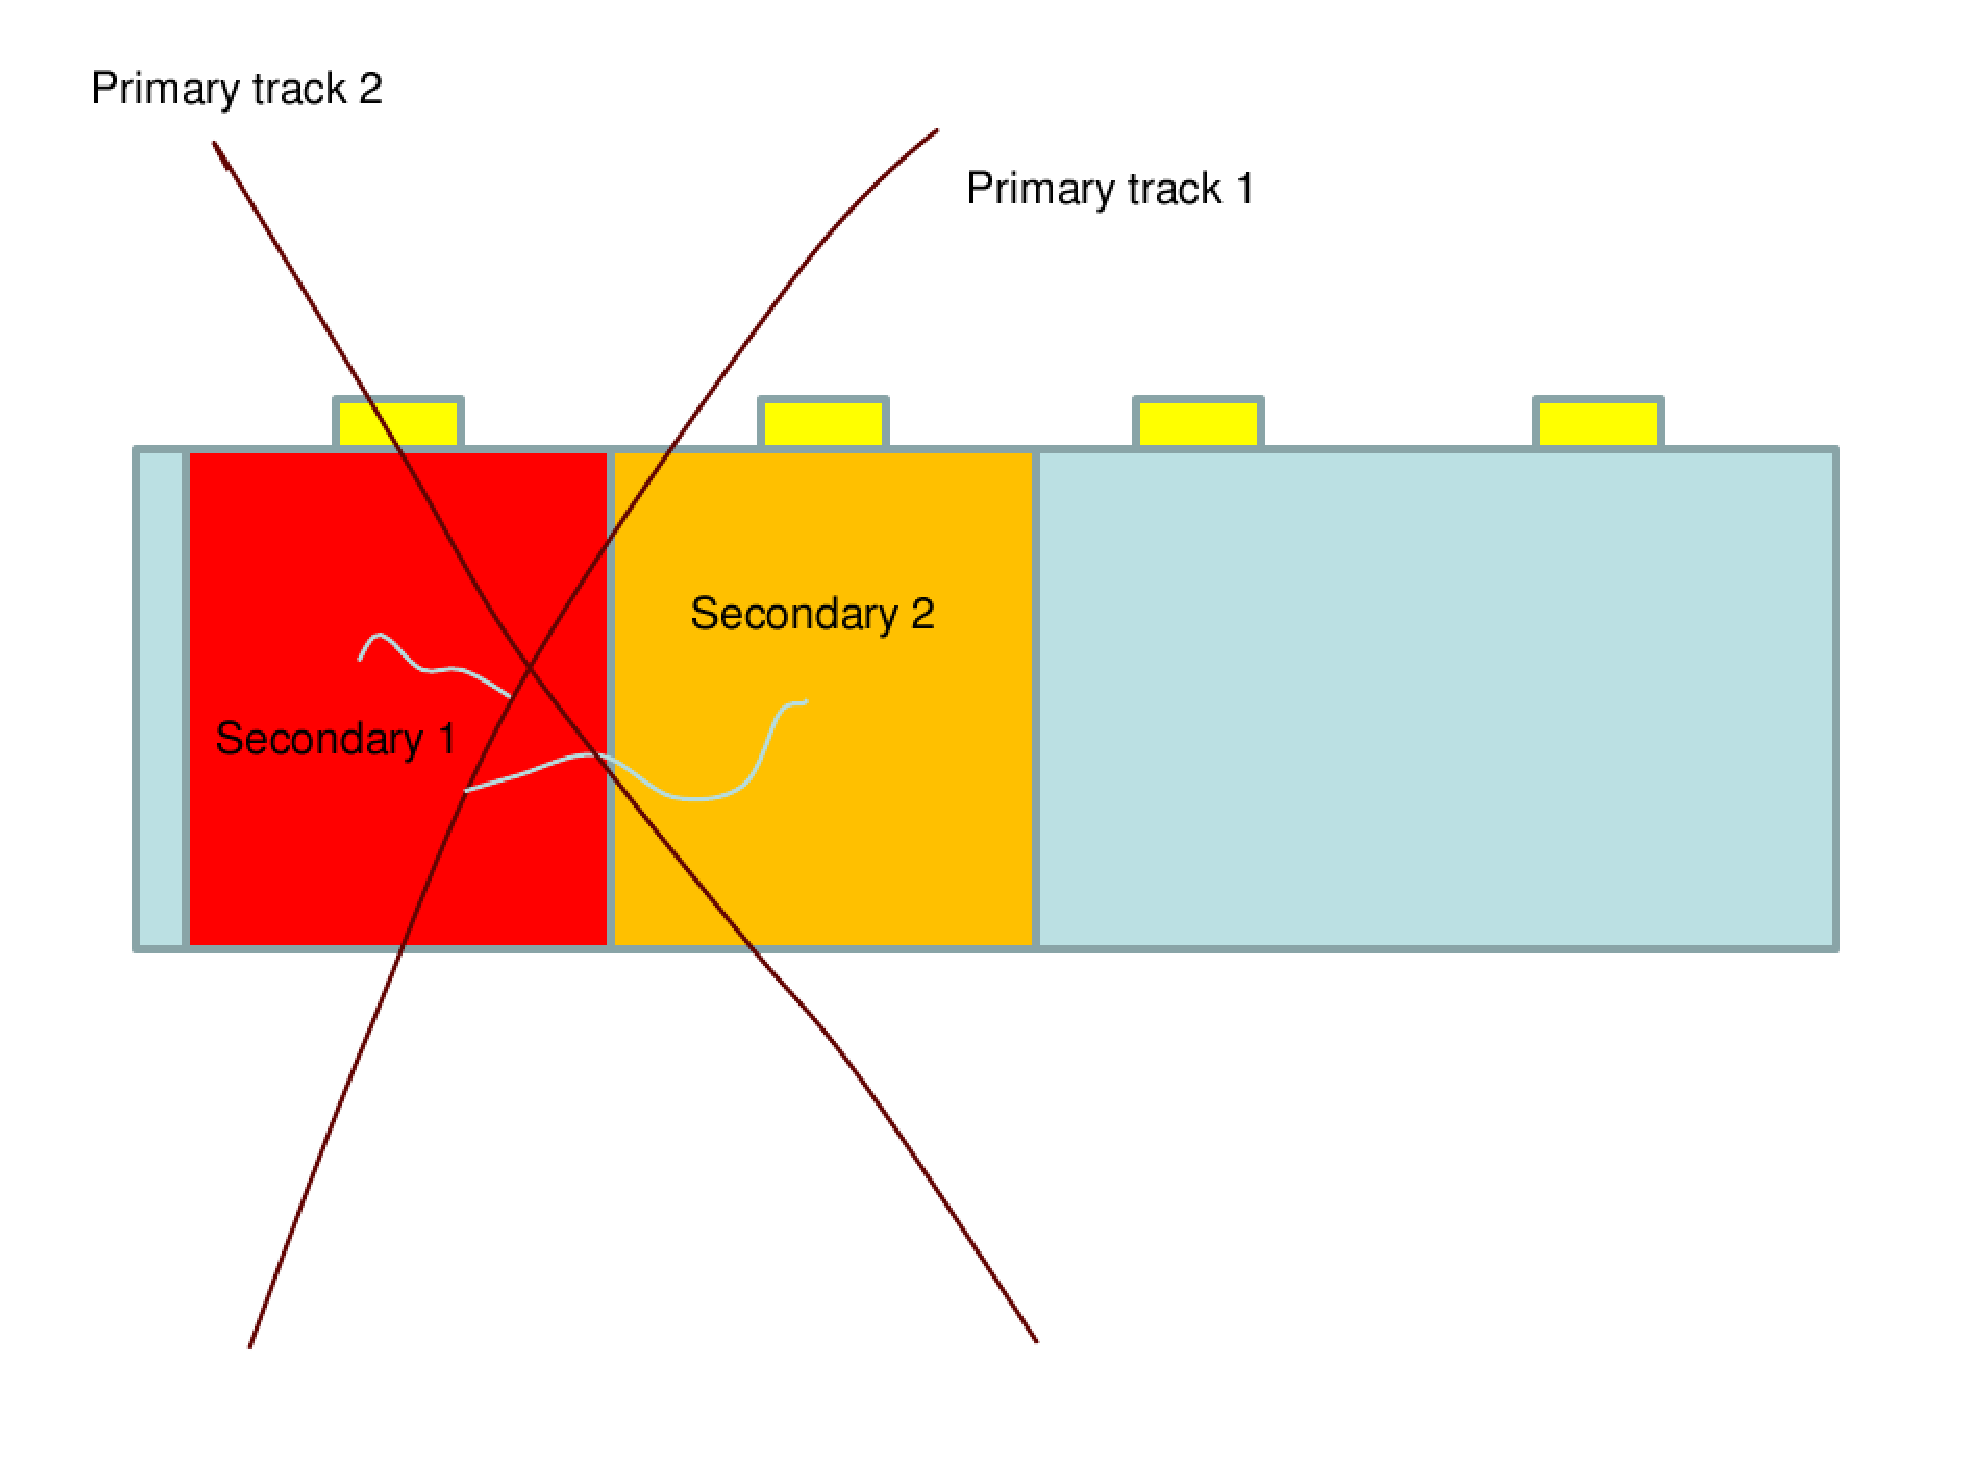
\epsfig{file=hit.eps, width=14.0cm,height=11cm}
\caption{\small{Hit definition illustration: In the picture two different 
detector elements are shown in different colors (red and orange). All 
tracks within the same TW and the same cell constitute one hit for that cell.
If any track has enough time separation from an existing hit, it will form 
another, separate hit.}}
\label{fig:hit_def}
\end{center}
\end{figure}
%%%%%%%%%%%%%%%%%%%%%%%%%%%%%%%%%%%%%%%%%%%%%%%%%%%%%%%%%%%%%%%%%%%%%%%%

\paragraph{Hit Process Factory}

~~

\vskip 0.3cm

Each detector has a custom Hit Process Routine (HPR) associated with it. 
The {\tt gemc} HPR pure virtual method is used to derive all the detector 
routines, and all HPRs are registered at run-time by a factory method.

The input to all HPRs is a {\tt gemc hit}. This stores, for each step in the 
hit, the following information:

\begin{itemize}
\item Hit Position (global coordinates);
\item Hit Position (relative to the volume in which the step occurs);
\item Deposited energy;
\item Time of the hit;
\item Momentum of the track;
\item Energy of the track;
\item Primary vertex of track;
\item Particle ID;
\item G4Track ID;
\item Identity;
\item Detector hit;
\item Mother particle ID;
\item Mother G4Track ID;
\item Mother primary vertex of track;
\item Energy threshold of the sensitive detector.
\end{itemize}

Each HPR processes the {\tt gemc} hit and produces STL vectors of double 
(raw information) and integers (digitized informations).  Each vector 
corresponds to a MySQL entry in the bank table corresponding to the HPR. 

\paragraph{Elements Identity}

~~

\vskip 0.3cm

In order to correctly identify and process the correct detector 
element at run time, a class {\tt identifier} is used.  The following 
scenarios can happen:

\begin{itemize}

\item[1)] For detectors where each element corresponds to a unique volume, 
the identifier remains unchanged.
\item[2)] For detectors where each element corresponds to a unique volume 
that is copied, the identifier copy number is determined at run time.
\item[3)] For detectors where different elements correspond to the same 
volume, the identifier is processed at run-time by the identifier method of 
the Hit Process Routines described above. For example, in the Drift Chamber 
implementation the single cells are not GEANT4 volumes (due to the fact that 
there are too many of them).  The sensitive volumes are instead layers of gas. 
At run-time, the cell is identified by the HPR based on the track position in 
each layer.
\end{itemize}

\paragraph{Output}

~~

\vskip 0.3cm

\noindent
The file formats for the simulation output stream are registered in {\tt gemc} 
by a factory method. New files types can be derived from the c++ pure virtual 
methods defined in {\tt gemc}. The main registered formats, selectable at 
run-time, are:

\begin{itemize}
\item txt: readable from any editor or shell. Bank names, variables are 
printed out.
\item EVIO: this is the format used by the CODA system, and unanimously 
chosen to be the default format for the output stream. Banks and variables 
are identified by integers (tag and num) defined in the MySQL tables.
\end{itemize}

The EVIO output can be viewed with the utility evio2xml, that outputs events 
in XML format.

\paragraph{Doxygen Documentation}

~~

\vskip 0.3cm

The c++ code is documented with doxygen. The documentation can be found at:

\begin{verbatim}
        http://clasweb.jlab.org/clas12/gemc_doxygen
\end{verbatim}

\paragraph{Results}

~~

\vskip 0.3cm

A sample event is shown in Figure \ref{gemcevent1}.
In the right-hand panel a single electron at $\theta = 10^\circ$ and $\phi = 0^\circ$ with momentum $p = 8~\rm GeV$ is simulated.
The left-hand panel shows the graphical user interface that allows the user to control the simulation.
Major components that remain to be added are the forward Cerenkov counters and the preshower calorimeter (PCAL) located in front of the existing electromagnetic calorimeter.
The code has a built-in event generator and the capability to read in an event file in the LUND format.
It has been built and runs on several linux distributions, Mac, and Windows Vista.
Additional tools are gemc\_evio2root (converts gemc output files in EVIO format to ROOT trees) and gevio (reads the EVIO output files from gemc).
Documentation can be found at the CLAS12 Software wiki:

\begin{verbatim}
        http://clasweb.jlab.org/wiki/index.php/CLAS12_Software
\end{verbatim}

%%%%%%%%%%%%%%%%%%%%%%%%%%%%%%%%%%%%%%%%%%%%%%%%%%%%%%%%%%%%%%%%%%%%%%%%
\begin{figure}[htb]
\begin{center}
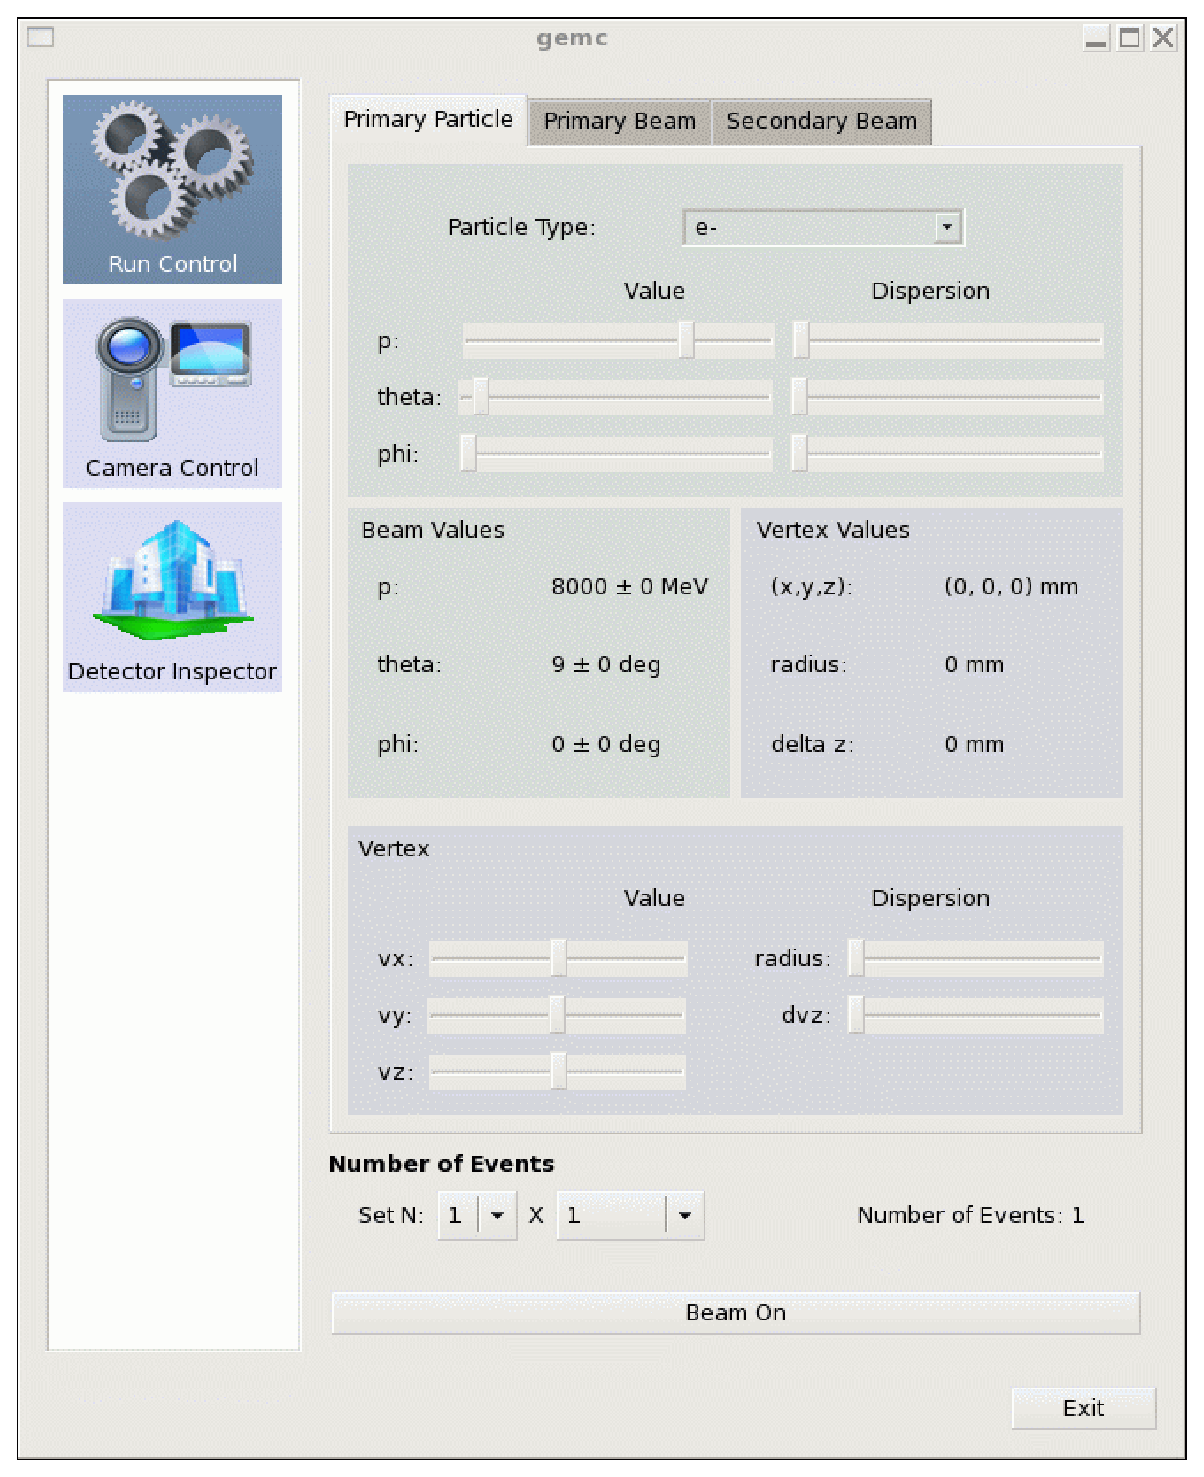
\includegraphics[height=3.0in]{gemcgui1.ps}\hspace{0.2in}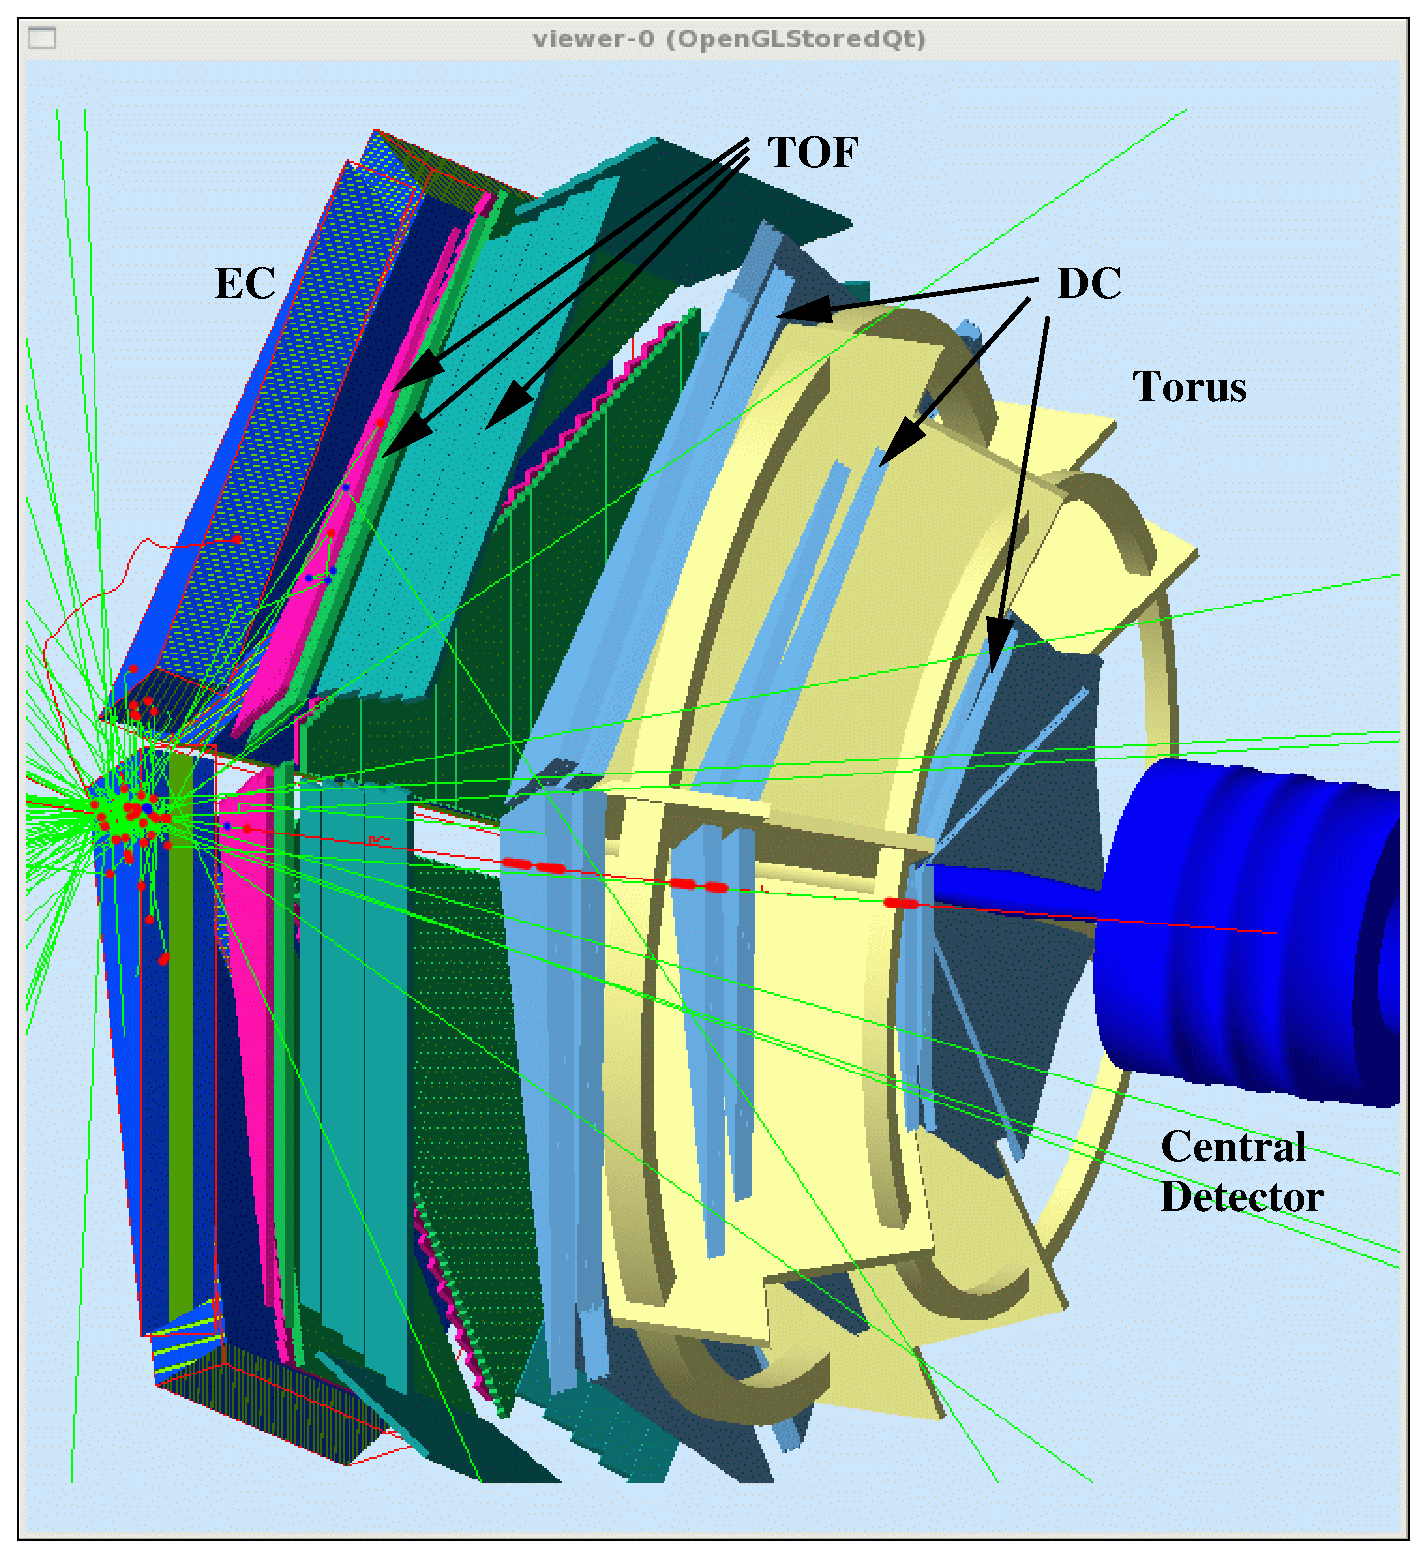
\includegraphics[height=3.0in]{gemcevent2.eps}
\caption{A simulated event in gemc. In the right-hand panel red tracks represent the scattered electron and other charged particles. Green tracks represent
neutral particles which are typically photons here. Red points represent hits in individual detectors, {\it e.g.} scintillator 
strips in the calorimeter. The graphical user interface that controls the simulation is shown in the left-hand panel.}\label{gemcevent1}
\end{center}
\end{figure}
%%%%%%%%%%%%%%%%%%%%%%%%%%%%%%%%%%%%%%%%%%%%%%%%%%%%%%%%%%%%%%%%%%%%%%%%

Some preliminary results for the CLAS12 electromagnetic calorimeter (EC) simulated with gemc are shown in Figure \ref{gemcECresults}.
The left-hand panel shows the results for the sampling fraction (the ratio of the energy measured from the calibrated light production to the electron energy) as a function 
of electron momentum for 
electrons at  $\theta = 10^\circ$ and $\phi = 0^\circ$ (blue points).
The gemc results are compared with the expectation for the calorimeter in the original CLAS6 EC \cite{ref:ECnim}. We are reusing the CLAS6 EC in CLAS12 so we expect the blue points to
roughly match the curve. There will be differences between the two because the CLAS12 EC analysis is preliminary and the electrons pass through different
materials before they reach the EC in the two detectors.
The right hand panel shows the simulated energy resolution of the EC as a function of electron momentum. 
The black curve shows the expectation for the EC in the CLAS6 configuration
and blue points are the result of the gemc simulation.
Again, the gemc results are preliminary, but agree with the CLAS6 results at the 10-15\% level.
%%%%%%%%%%%%%%%%%%%%%%%%%%%%%%%%%%%%%%%%%%%%%%%%%%%%%%%%%%%%%%%%%%%%%%%%
\begin{figure}[htb]
\begin{center}
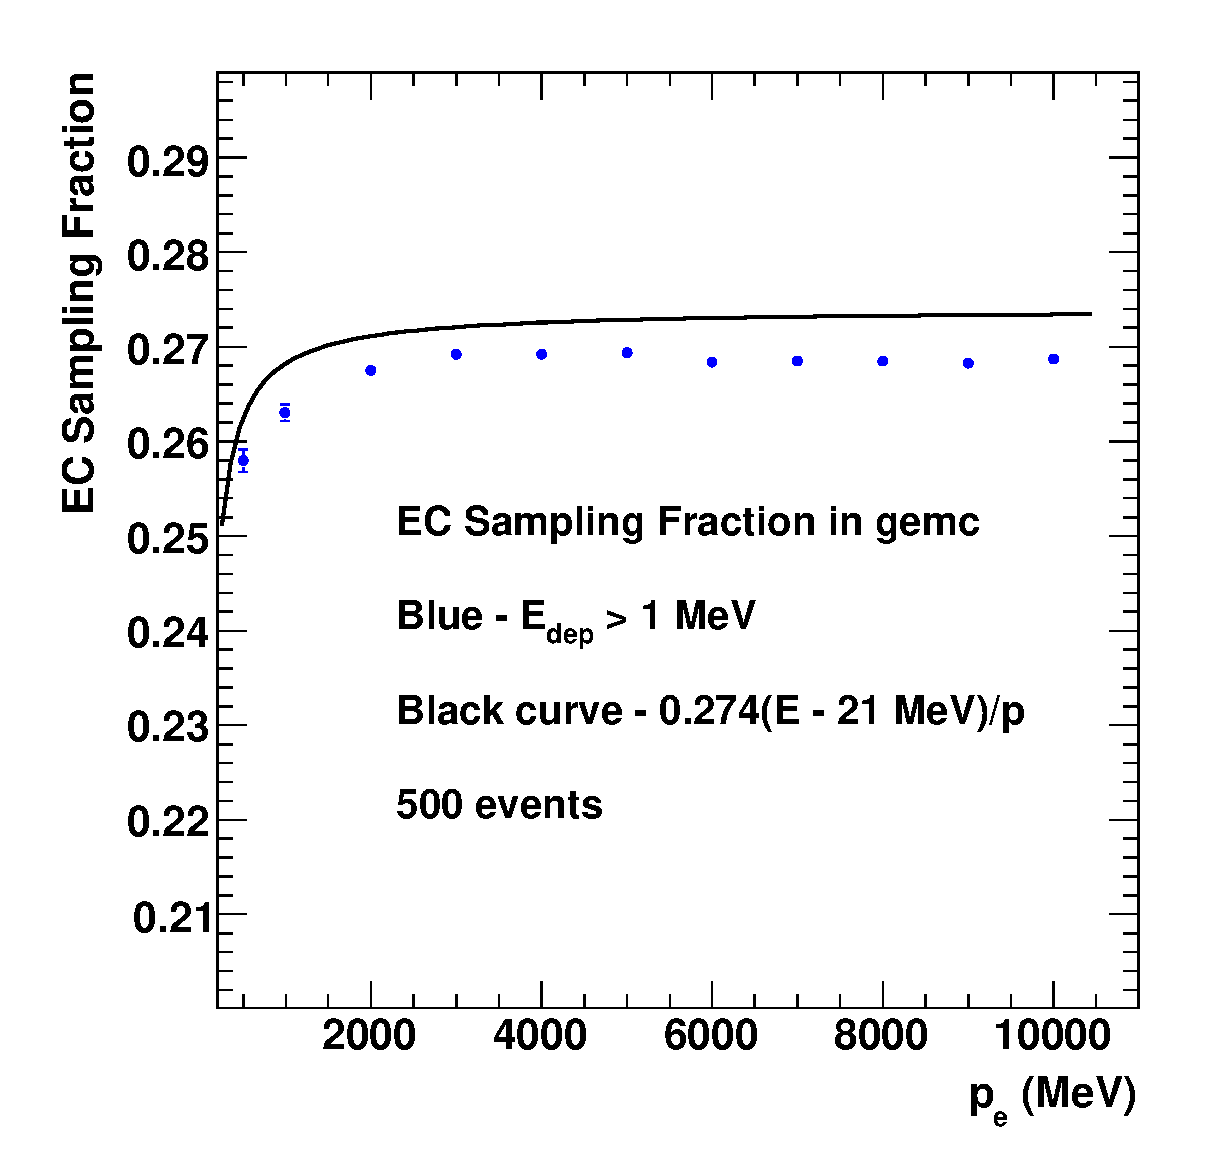
\includegraphics[height=3.0in]{sf3.eps}\hspace{0.2in}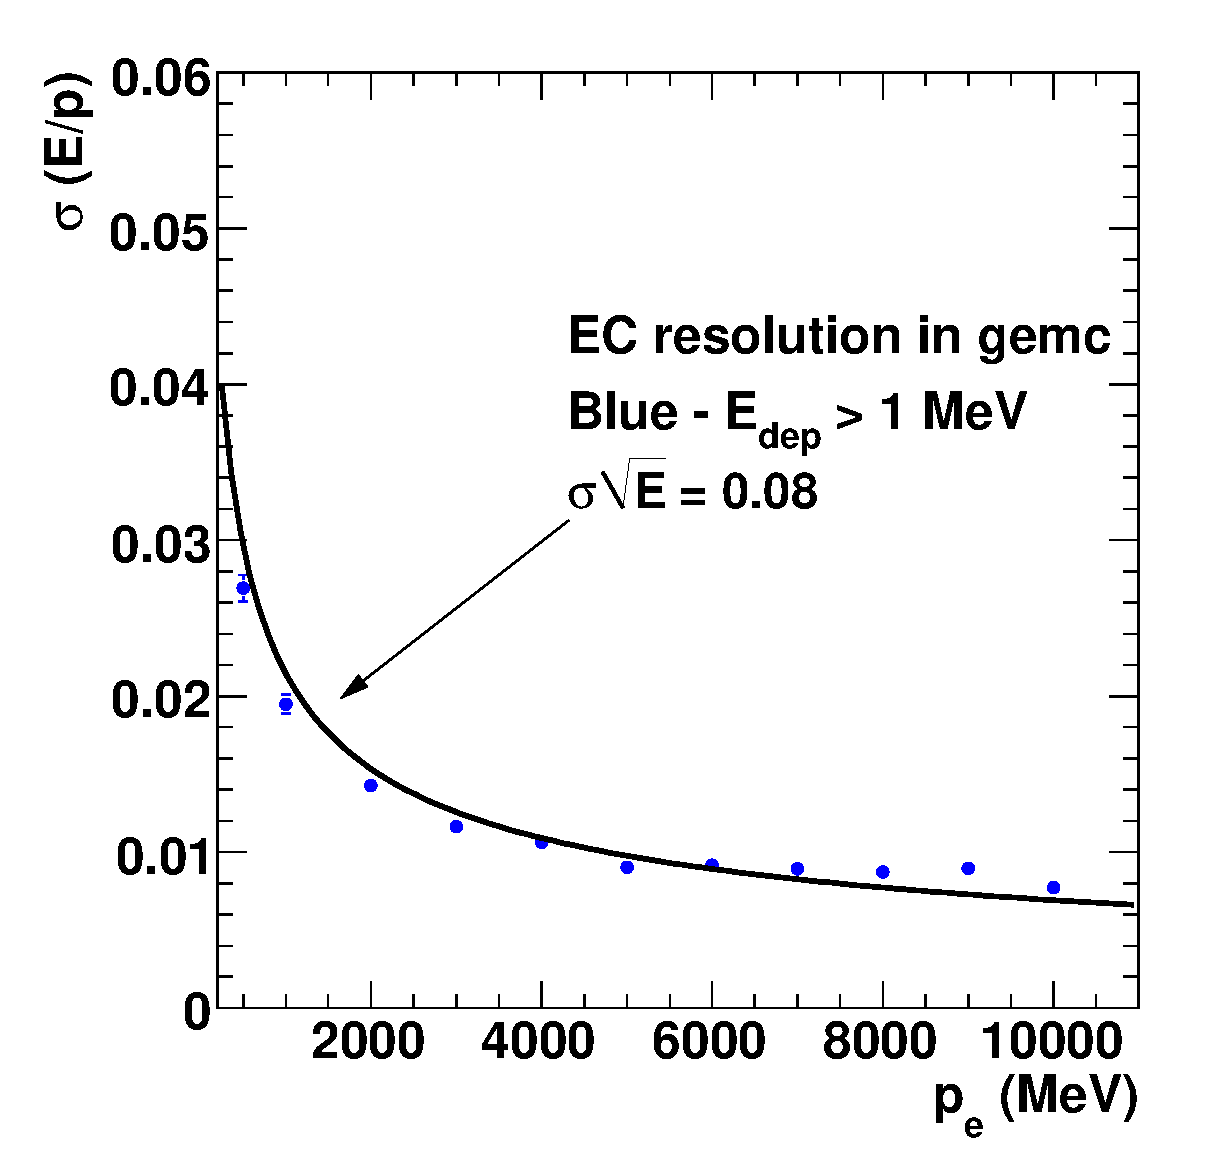
\includegraphics[height=3.0in]{res3.eps}
\caption{EC results from gemc. The left-hand panels shows a comparison of gemc results (blue points) for the sampling fraction and a semi-empirical calculation for the CLAS6 EC.
The right-hand panel shows the momentum resolution simulated with gemc (blue points) compared with the CLAS6 results (black curve). }\label{gemcECresults}
\end{center}
\end{figure}
%%%%%%%%%%%%%%%%%%%%%%%%%%%%%%%%%%%%%%%%%%%%%%%%%%%%%%%%%%%%%%%%%%%%%%%%



\subsection{The {\tt CLAS12} Fast Monte Carlo}

Detailed detector simulation and reconstruction of physics events in 
{\tt CLAS12}, based on GEANT4, is very CPU intensive and hence time 
consuming due to the high energy and multiplicity of the Monte-Carlo events 
and the complexity of the detectors.  A dynamically configurable package for
fast Monte-Carlo simulation and reconstruction (FASTMC) has been developed 
for {\tt CLAS12} to allow fast studies of effects of detector resolutions 
and acceptances on various samples of Monte-Carlo events.  Each step of the 
chain -- simulation and track reconstruction -- has been replaced by modules 
that parameterize the acceptance and responses of the different detector 
components.

The FASTMC package uses a configuration file provided by the user, which 
has all relevant information, including the resolutions and acceptances for 
different particles and kinematics.  The initial set of parameters was 
derived from calculations and are getting updated with new simulation 
studies from GEANT4 {\tt CLAS12} simulations.  Sets of parameters were 
defined for the central and forward detectors of {\tt CLAS12} and for inbending
(torus current positive, so electrons will bend in toward the beam axis) 
and outbending conditions.  Two subroutines were called in the FASTMC package 
subsequently to provide information on acceptance, along with momentum 
and angular smearing of tracks in {\tt CLAS12}. 

\subsubsection{{\tt CLAS12} Acceptance}

The parameters defining the acceptance of events are listed in the 
configuration file.  The computed acceptance of $ep \to e\pi X$ events is 
shown in Fig.~\ref{fig:accept}.

%%%%%%%%%%%%%%%%%%%%%%%%%%%%%%%%%%%%%%%%%%%%%%%%%%%%%%%%%%%%%%%%%%%%%%%%
\begin{figure}[htbp]
\centering
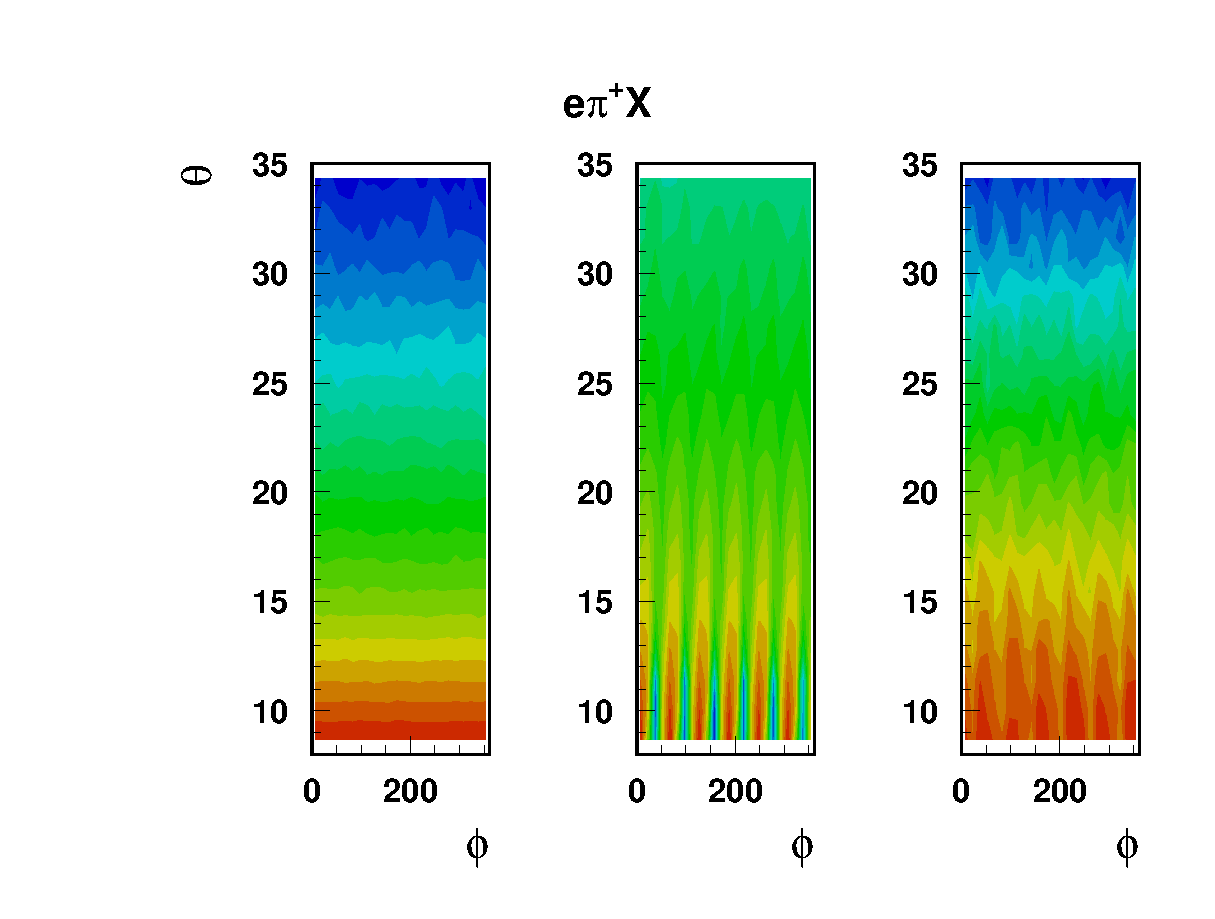
\includegraphics[width=4in]{drawcl12thetavsphi.elepim.log.eps} 
\caption{\small{{\tt CLAS12} acceptances for generated DIS electrons (left), 
reconstructed electrons (center), and reconstructed $\pi^+$ (right).}}
\label{fig:accept}
\end{figure}
%%%%%%%%%%%%%%%%%%%%%%%%%%%%%%%%%%%%%%%%%%%%%%%%%%%%%%%%%%%%%%%%%%%%%%%%

\subsection{{\tt CLAS12} Momentum and Angular Smearing}

The parameters defining the smearing of particle angles and momenta 
are listed in the configuration file.  The resolutions are calculated 
using simple parameterizations obtained from the GEANT4 simulation for 
momentum, polar, and azimuthal angles using:

\begin{equation}
\sigma_p =  \frac{T_{max}}{T} \sqrt[]{(\sigma_1^p \cdot p)^2 + 
\left( \frac{\sigma_2^p}{\beta} \right)^2}
\end{equation}

\noindent
where,

\begin{equation}
\sigma_{[1/2]}^p = \sigma_{[{1/2}]}^1 + \sigma_{[{1/2}]}^2 \cdot \theta 
+ \sigma_{[{1/2}]}^3 \cdot \theta^2,
\end{equation}

\begin{equation}
\sigma_\theta=\sqrt{\sigma_{1\theta}^2
+(\sigma_{2\theta}/p/\beta)^2}\sin^2\theta,
\end{equation}

\begin{equation}
\sigma_\phi=\sqrt{\sigma_{1\phi}^2+(\sigma_{2\phi}/p/\beta)^2}.
\end{equation}

The smearing due to energy loss and multiple scattering of particles in 
the central detector is shown in Fig.~\ref{fig:smear}.

%%%%%%%%%%%%%%%%%%%%%%%%%%%%%%%%%%%%%%%%%%%%%%%%%%%%%%%%%%%%%%%%%%%%%%%%
\begin{figure}[htbp]
\centering
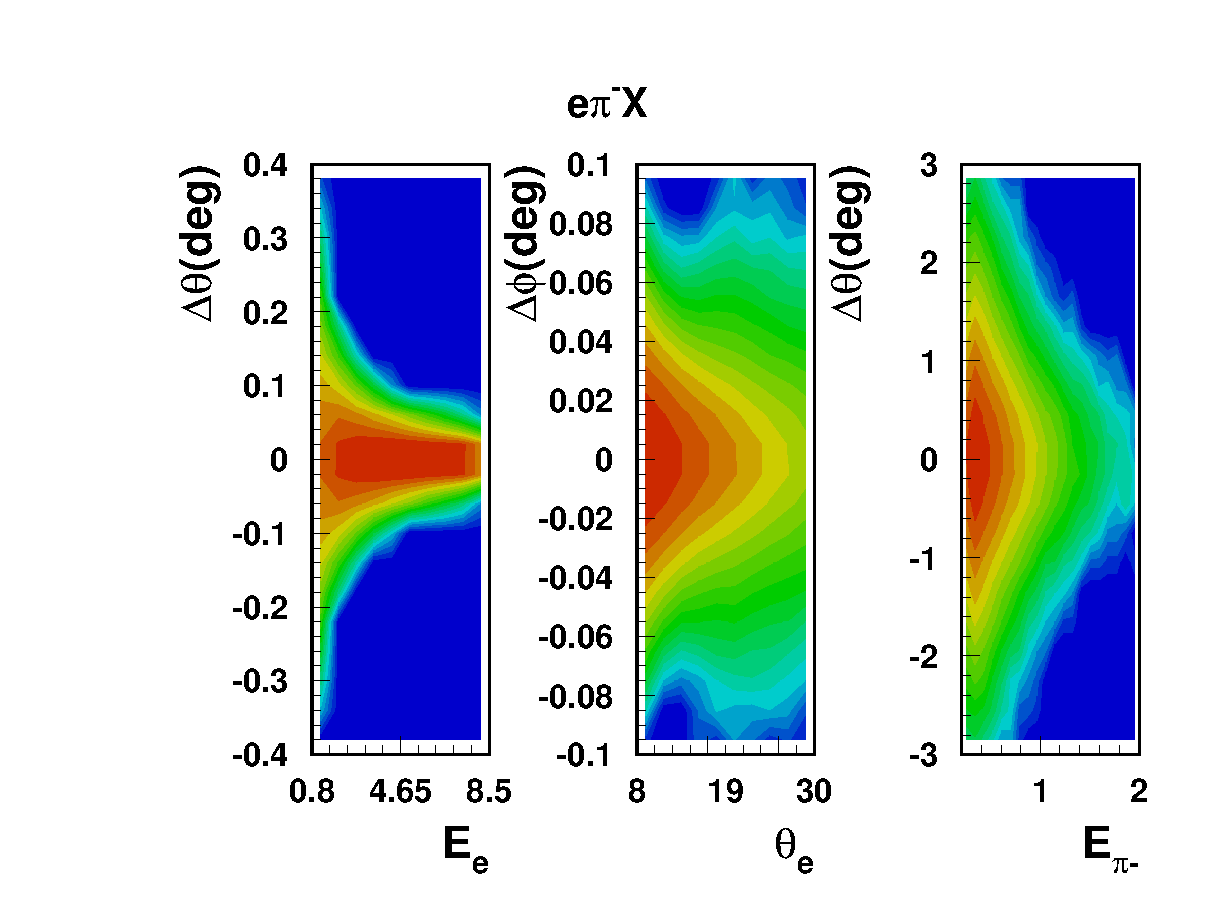
\includegraphics[width=5in]{drawcl12dthetavs.epi.log.eps} 
\caption{\small{Resolutions of electron polar (left) and azimuthal (center) 
angles in the forward detector and $\pi^-$  in the central detector (right).}}
\label{fig:smear}
\end{figure}
%%%%%%%%%%%%%%%%%%%%%%%%%%%%%%%%%%%%%%%%%%%%%%%%%%%%%%%%%%%%%%%%%%%%%%%%

FASTMC allows study of the effects of detector resolutions and smearing on 
various physics observables. The missing mass resolution of the reaction 
$ep \to e\pi X$ is shown in Fig.~\ref{fig:epX}.  The distribution of events 
from $\Lambda$ and $\Sigma$ decays as a function of the angle between planes 
containing the $\Lambda$ and the $K$ are shown in Fig.~\ref{fig:KLam}.
Fig.~\ref{fig:twopi} shows the $W$ distribution for a two pion production
reaction calculated from the electron momentum and using detected pions in 
the forward and central detectors. 

%%%%%%%%%%%%%%%%%%%%%%%%%%%%%%%%%%%%%%%%%%%%%%%%%%%%%%%%%%%%%%%%%%%%%%%%
\begin{figure}[htb]
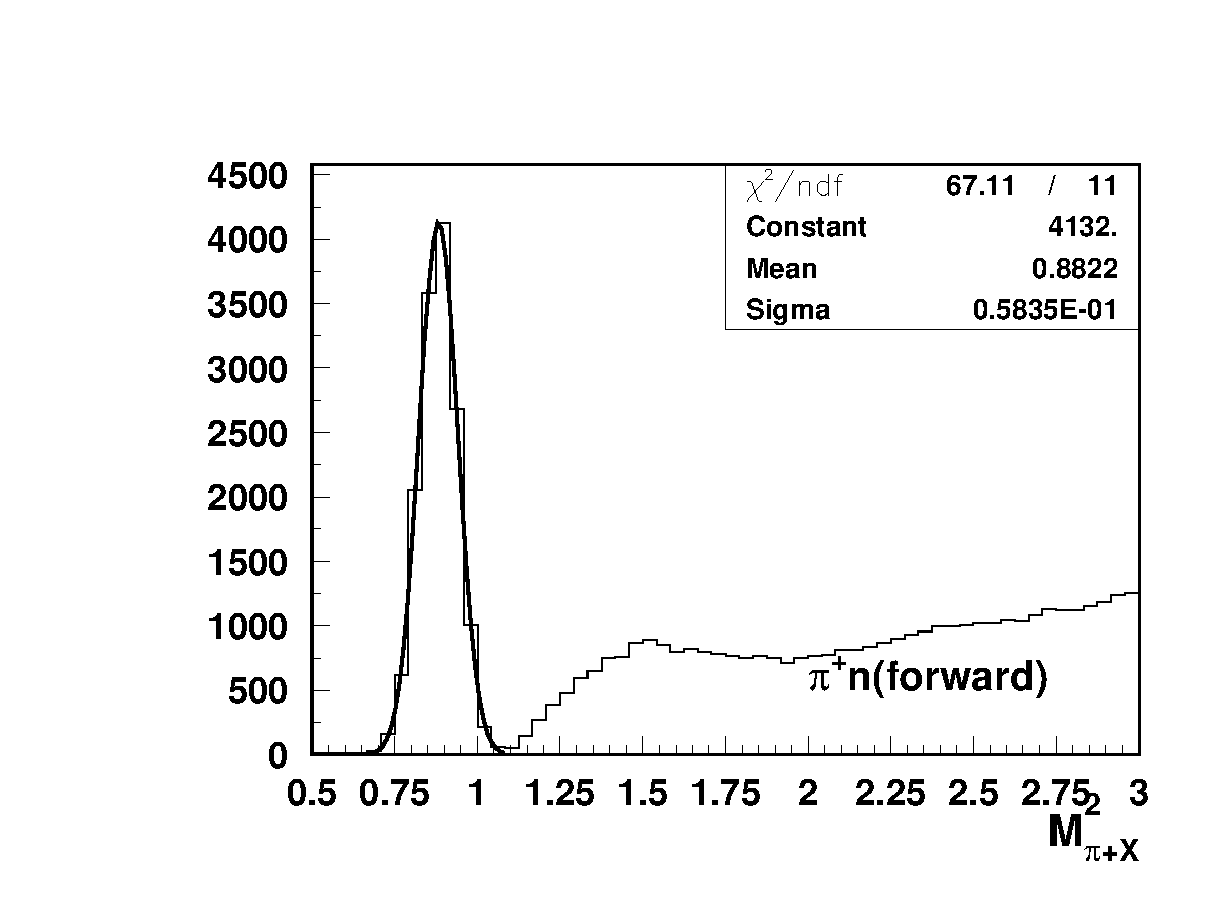
\includegraphics[width=3in]{pipmx.forw.eps}
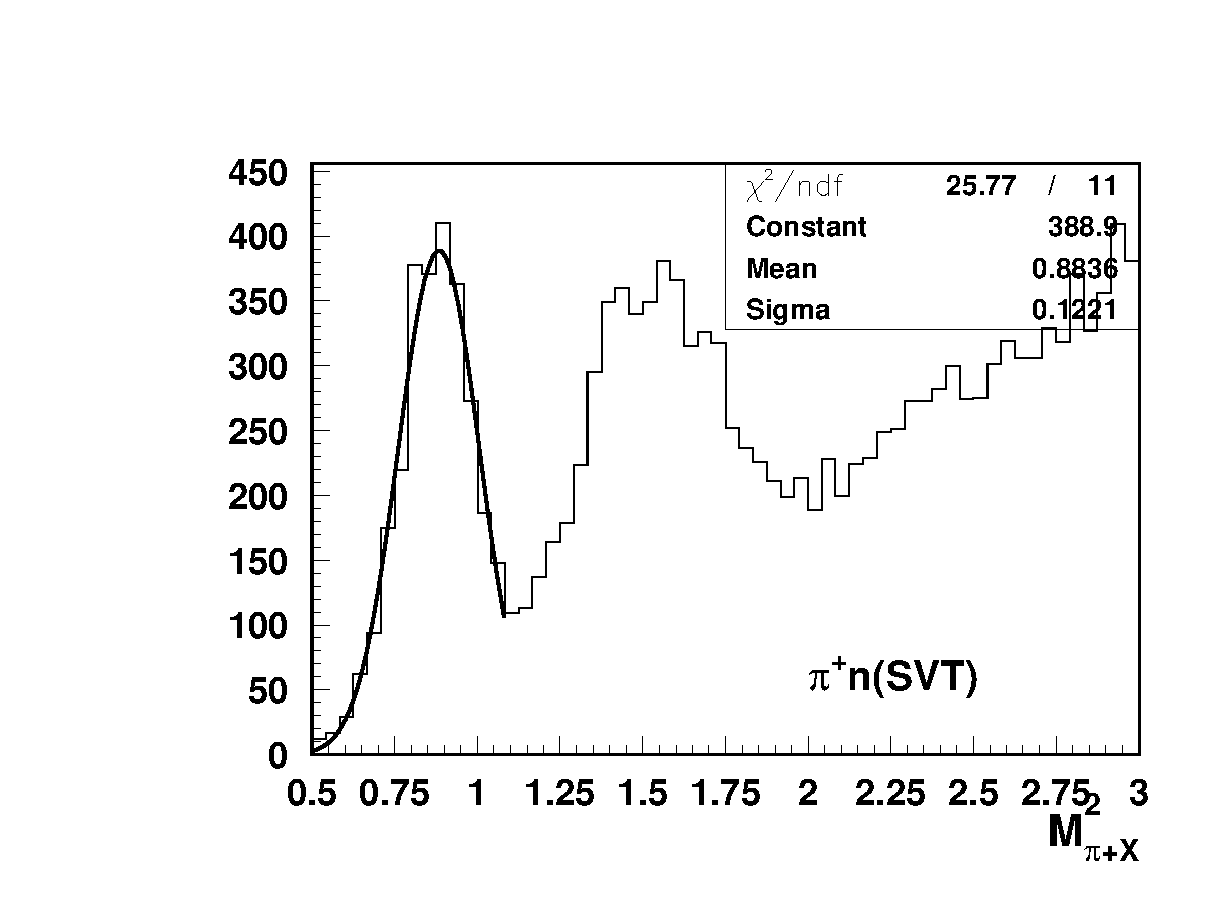
\includegraphics[width=3in]{pipmx.cent.eps}
\caption{\small{Missing mass resolution for $ep \to e'\pi X$ for forward  
(left) and large angle $\pi^+$ (right) events.}}
\label{fig:epX}
\end{figure}
%%%%%%%%%%%%%%%%%%%%%%%%%%%%%%%%%%%%%%%%%%%%%%%%%%%%%%%%%%%%%%%%%%%%%%%%

%%%%%%%%%%%%%%%%%%%%%%%%%%%%%%%%%%%%%%%%%%%%%%%%%%%%%%%%%%%%%%%%%%%%%%%%
\begin{figure}[htb]
\begin{minipage}[b]{6.0cm}
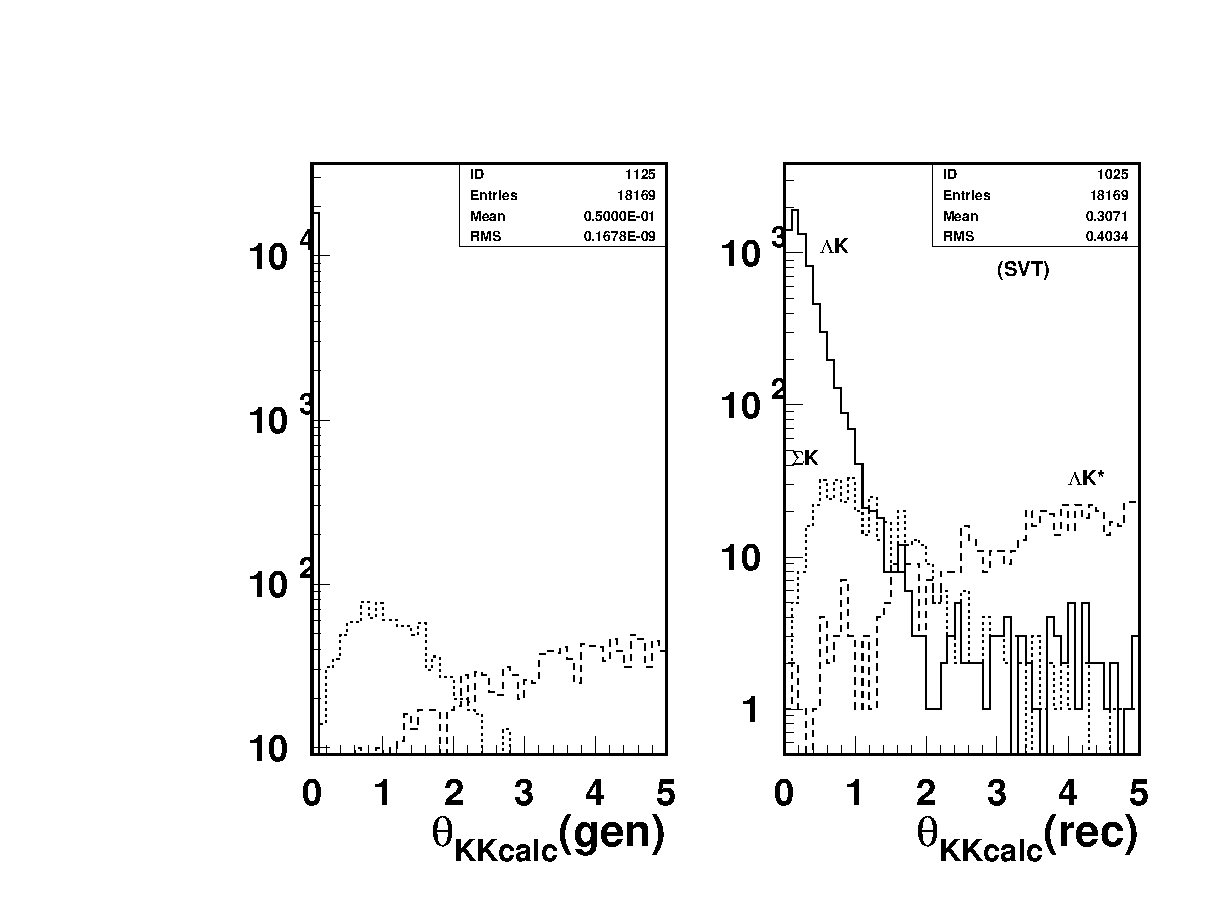
\includegraphics[width=3in]{lambdakaonmak.lam.tmax5.eps}
\end{minipage}
    \ \hspace{0mm} \hspace{0mm} \
\begin{minipage}[b]{6.0cm}
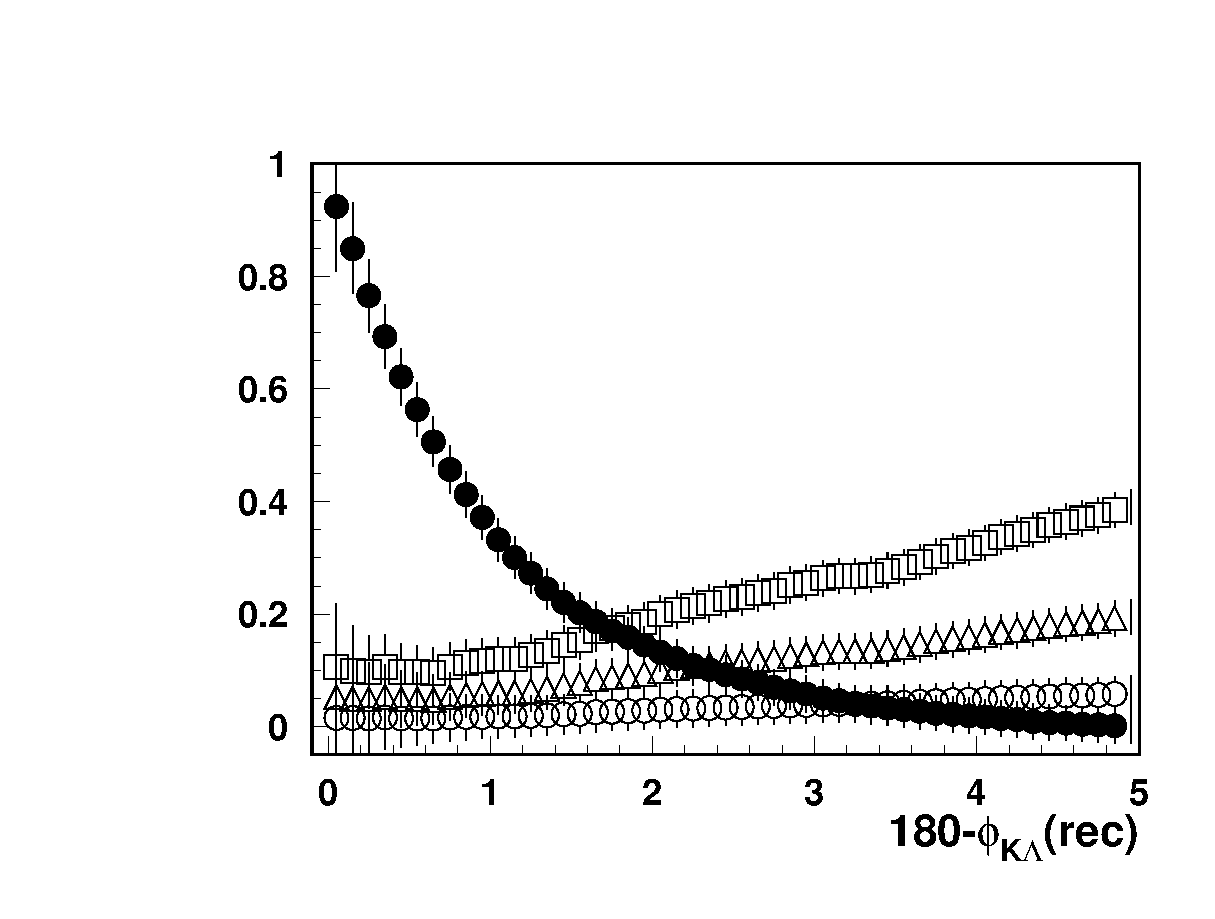
\includegraphics[width=3in]{lambdakaon-sepppl.lam.tmax5.eps}
\end{minipage}
\caption{\small{Angle between the $\Lambda$ and the $K$ for different 
processes for generated (left) and reconstructed (middle) distributions. 
The right panel shows the corresponding efficiencies (circles) as a 
function of a cut on that angle and the corresponding contamination 
(triangles).}}
\label{fig:KLam}
\end{figure}
%%%%%%%%%%%%%%%%%%%%%%%%%%%%%%%%%%%%%%%%%%%%%%%%%%%%%%%%%%%%%%%%%%%%%%%%

%%%%%%%%%%%%%%%%%%%%%%%%%%%%%%%%%%%%%%%%%%%%%%%%%%%%%%%%%%%%%%%%%%%%%%%%
\begin{figure}[htb]
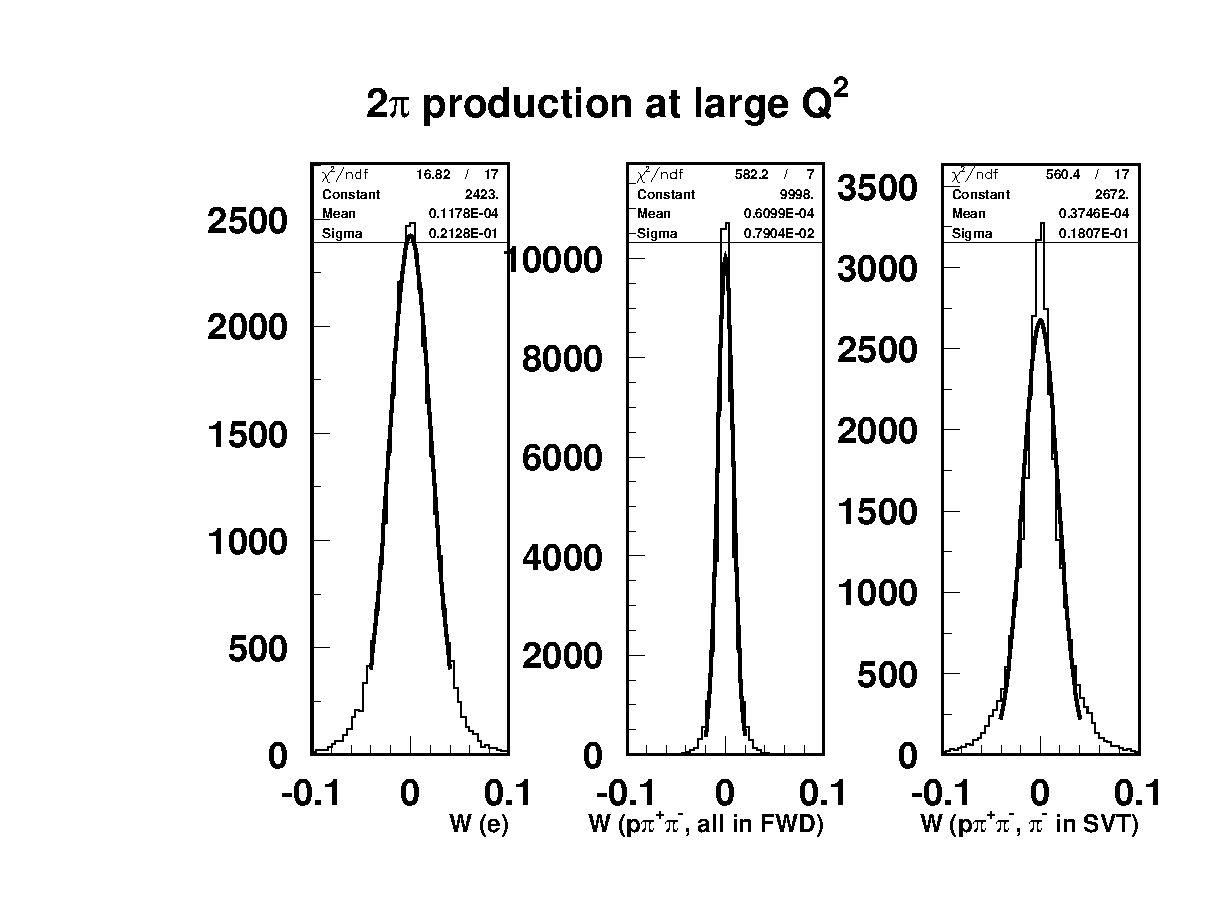
\includegraphics[width=6in]{twopi.eps}
\caption{\small{$W$ distributions for exclusive two pion processes in 
{\tt CLAS12} from FASTMC. $W$ computed from the electron (left), the
detected pions in the forward detectors (middle), and the detected pions 
in the central detectors (right).}}
\label{fig:twopi}
\end{figure}
%%%%%%%%%%%%%%%%%%%%%%%%%%%%%%%%%%%%%%%%%%%%%%%%%%%%%%%%%%%%%%%%%%%%%%%%

\section{Event Reconstruction}

The main goal of the event reconstruction program is to provide track 
parameters and particle identification on an event basis, to any physics 
analysis. These events will in practice either come from real data or 
from the Monte Carlo simulation.  The reconstruction program should also 
be able to perform specific tasks, like sending hits and corresponding fit 
results to the event display service. 

\subsection{Socrat}

This program is currently developed in 
c, but will eventually be coded in c++, with an object oriented structure and modified to take advantage of multi-threaded processors. 
Even if the tracking techniques (track finding and track fitting) can be 
used in a detector-independent form, their implementation will be adapted 
to the geometry of the {\tt CLAS12} spectrometer, and therefore split in 
two parts:

\vskip 0.2cm

{\it Central Tracking:} this part provides the reconstruction of particles 
detected in the Silicon Vertex Tracker, located inside the high magnetic 
field of the solenoid. Due to the approximate $\phi$ symmetry of this 
region, we implemented a Kalman Filter algorithm using cylindrical 
coordinates. A track finding procedure has also been developed to separate 
real tracks from the background.

{\it Forward Tracking:} particles produced at small angles are detected in two 
different subsystems, the Forward Vertex Tracker and the Drift Chambers. A 
key issue of the tracking program is to provide an algorithm that will 
efficiently match track segments found in these detectors, in the presence of 
background.  As for the central part, we also implemented a Kalman Filter 
algorithm.

\vskip 0.2cm

The last task of the tracking program will be to link tracks found in these 
two regions, that will include a vertex fitting algorithm, thus providing a 
full event reconstruction.  Different outputs (not only the structure, but 
also the contents) will be produced, depending on the incoming request.

\subsection{Tracking in Java (jSocrat)}

As described above, tracking in CLAS12 is done in three detectors, the Drift Chambers (DV), and the Forward and Barrel regions of the Silicon Vertex Tracker.  Event detector information is passed to the tracking program, {\it jSocrat}, via the standard EVIO file format. {\it jSocrat}  contains two separate components:  forward and central tracking.  Central tracking deals with the barrel region of the SVT, while forward tracking connects the forward region of the SVT with the drift chambers.  The central and forward tracking can be run independently from one another, and therefore designed to be run on separate threads.
{\it jSocrat} is largely based on Sebastien Procureur�s program, Socrat, developed within the CERN Root C-Interpreter, and borrows most of the algorithms from Socrat. 
Hit-linking in the forward tracking is accomplished separately for the drift chamber and the forward SVT.  In the drift chamber, the task is to find tracks among the hits:  first, grouping hits within each superlayer to form �clusters�, then linking pairs of clusters to produce �segments�, and then linking the �segments� together to produce tracks.  Using similar criteria, track segments are also constructed by hits in the forward SVT.  (For a more detailed description of the algorithms, see the javadoc of jSocrat in the CLAS12 source code repository). 
For each of the tracks found in the DC, a Kalman filter is run to calculate the track .  During the Kalman filter, the path is tracked through the magnetic field backwards from the DC, until the track reaches the plane of intersection with the closest plane of the FSVT.  The nearest FSVT track segment to the extrapolated track is used for continuing the tracking as far upstream as possible.
The process is similar for the central tracking.  The barrel SVT hits are linked together to form strip intersections.  Then these intersections are linked together to form tracks.  For each track, intersection positions are recalculated using a helical approximation that utilizes the other three (or two) intersections in the track.  (For a more detailed description of the algorithms for the BSVT, see the javadoc of jSocrat in the CLAS12 source code repository).   This is done to get a better estimate of where the particle hit the strips in the BSVT. Then, a Kalman filter is used for estimating the tracking parameters.  Because the track has to be swum backwards a shorter distance in the central tracking than in the forward tracking, the Kalman filter algorithm for the central tracking takes less time.  Both Kalman filters use the same time-step. 

The most time-consuming task in jSocrat is running the Kalman Filter on the forward tracks.  The Kalman filter can thus be multi-threaded.  In the Kalman filter, jSocrat utilizes the Clas12 detector�s field map files, which it loads in at start time from a query to the Magnetic Field Service.  

	The output in jSocrat is an EVIO file, the banks of which are described in the javadocs of jSocrat.

Currently, vertex finding is being developed.


\section{On-Line Software}

During the actual data-taking periods of {\tt CLAS12}, it is of course 
expected that there will be full construction of a {\it significant} fraction 
of the acquired data.  Such analysis insures that the data is of expected 
quality, and permits monitoring of the individual detectors from a different 
perspective than just hardware readout, such as wire profiles, ADC spectra, 
etc..  Experimenters should expect they should also be able to monitor the 
performance of the {\tt CLAS12} detector by examining the specific events and 
physics parameters under study.  This capability will require {\it full} event 
reconstruction. 

In addition, some reconstruction analysis can be utilized as a Level-3 
trigger to filter unwanted events from the data stream, thus minimizing 
storage, bandwidth, and other precious resources.

The entire suite of services will be available to the online and data 
acquisition system, either directly as network available resources, or as 
shared code. 

\section{Code Development and Distribution}

\subsection{Code Management}

For {\tt CLAS12}, we have elected to use the widely adopted and free (open 
source) subversion revision control system. Subversion is the open source 
software community's replacement for cvs. It has many of the same features 
and employs the same no-lockout paradigm. (That is, conflicts are resolved 
through merging rather than avoided through code locks -- the latter 
generally found to be too draconian and a hindrance to productivity.) In 
addition, subversion plug-ins are available for the popular integrated 
development environments, such as the widely used eclipse. This allows one to 
check in, check out, track changes, and merge differences with mouse-clicks 
in a development environment rather than through a command line. 

In {\tt CLAS}, all users, whether or not they were developers, accessed the 
repository, downloaded code, and built scripts.  They then tried, with 
mixed results, to build the complex packages. We have abandoned that 
approach.  In {\tt CLAS12}, we have decided to implement a three-tiered code 
distribution system.  The first level will be access to the subversion 
repository. Only developers will access code in this manner. The second level 
will be code releases, in the form of archives, and intelligent build scripts 
that do not rely on environment variables. In {\tt CLAS}, the user wanting to 
use an application accessed the repository and downloaded the latest code, 
which may have included bugs checked in the night before. In {\tt CLAS12} the 
user will go to a web page and download a specific, tested released. A third 
tier of release, for limited systems (probably only for whatever Linux system 
JLab is supporting) is to distribute binaries.  This in an area in which we 
expect and have already obtained substantive student involvement.

\subsection{Code Release}

The consensus in the software group is to base our software process on what 
is known in the software community as agile programming. Part of agile 
programming is a rapid release schedule based on development cycles called 
sprints.  The exact frequency has not yet been determined, but the canonical 
sprint duration is one month: two weeks of development and two weeks of 
testing and bug fixing. So every month a new version of all software is 
released, typically with modest changes from the previous release. 
Functionality is to advance incrementally, as opposed to infrequent but 
massively different updates.

\subsection{Software Tracking}

The software group recognized that complicated software development is 
aided by requirements, task, and bug tracking. To this end, Christopher 
Newport University has deployed a web-based commercial package called 
Gemini for the {\tt CLAS12} effort. Gemini will allow us to enter projects 
corresponding to the main development efforts, such as {\tt gemc} 
for the GEANT4 simulation. Then resources (developers) are assigned to the 
project. The time development will match the code release sprint cycles. For 
the next cycle, the new tasks will be entered, as well as the bugs that have 
to be fixed.  Developers will enter estimates regarding the time it will take 
to complete the tasks and fix the bugs. Project managers can see if the 
estimated time fits with the cycle duration, if not they can adjust 
accordingly by postponing some tasks or adding new tasks.  Developers can log 
their time to a task or bug so as to develop better intuition for estimating. 
The subversion revision control system can be set up so that any code checked 
in must have a comment that ties it, by ID to a task or bug in Gemini.

\section{Quality Assurance}

The Service-Oriented Architecture is composed of many integrated services 
loosely connected.  The usual interaction between the consumer of a service 
and the supplier of the service is not direct: generally there will be 
several processes and a network in between. As a result, during an extended 
development process, there becomes a strong possibility of errors invading 
the code, rendering it either unusable or incorrect. Quality assurance of 
developing projects then becomes a major concern. 

The program being proposed is {\it extensive} suite checks to assure that 
every major release is thoroughly checked prior to being made available to 
the {\tt CLAS12} Collaboration.  In addition, at any level the individual 
code developer will be able to check {\it any} version against the standard 
suite. 

The suite of reconstruction standards will include three types of data. The 
first is {\it pure} simulation, that is Monte Carlo generated data through 
the {\tt CLAS12} detector {\it without} any detector resolution included.  
Reconstruction of this data set should return {\it exactly} what was input; 
any deviation is suspect and cause for special consideration. The next set 
of standard data will be a persistent Monte Carlo data set {\it with} full 
simulation, whose results should remain consistent with input parameters. 
Finally, varied sets of actual data, fully testing as completely as possible 
all aspects of the reconstruction software, will be utilized to track the 
code development. Of course, in all data types, performance in terms of 
compute resources and storage will also be tracked. Databases of performance 
results will be maintained as a service for comparison.

\section{Computing Resources}

Based primarily on experience from the 6~GeV {\tt CLAS} computing usage, 
estimates have been made for computing resources required from 2012 through 
turn-on in 2015 and through the year 2017.  These estimates are summarized in 
Table~\ref{tab:Compute}. 

%%%%%%%%%%%%%%%%%%%%%%%%%%%%%%%%%%%%%%%%%%%%%%%%%%%%%%%%%%%%%%%%%%%%%%%%
\begin{table}[htdp]
\begin{center}
\begin{tabular}{|l|c|c|c|c|c|c|}
\hline 
{\bf Year}  & 2012 & 2013 & 2014 & 2015 & 2016 & 2017  \\  \hline
{\bf Simulation} & & & & & & \\
CPU & 5.7E4 & 5.7E4 & 5.7E4 & 5.7E4 & 5.7E4 & 5.7E4 \\
Petabytes & 2 & 5 & 7 & 5 & 5 & 5 \\ \hline
{\bf DAQ }& & & & & & \\
Petabytes & 0 & 0 & 0  & 2.2 & 2.4 & 2.5 \\ \hline
{\bf Calibration}  & & & & & & \\
CPU & & & & & & \\ \hline
{\bf Reconstruction} & & & & & & \\
CPU & 0 & 0 & 0 & 7.8E3 & 8.4E3 & 9.1E3 \\
Petabytes & 2 & 5 & 7 & 12 & 12 & 13 \\ \hline
%{\bf Cost} & & & & & & \\
%Cost of Computers (\$K) & \$63 & \$13 & \$0 & \$6 & \$4 & \$0 \\
%Cost of tape (\$K) & \$135 & \$281 & \$309 & \$451 & \$393 & \$342 \\
%Budget (\$K) & \$198 & \$294 & \$309 & \$456 & \$397 & \$342 \\
\hline
\end{tabular}
\end{center}
\caption{\small{{\tt CLAS12} computing resources.}}
\label{tab:Compute}
\end{table}
%%%%%%%%%%%%%%%%%%%%%%%%%%%%%%%%%%%%%%%%%%%%%%%%%%%%%%%%%%%%%%%%%%%%%%%%
